
\documentclass{sigplanconf}[9pt]

\usepackage{amsmath}
\usepackage[T1]{fontenc}
\usepackage[utf8]{inputenc}
\usepackage{authblk}
\usepackage{proof-dashed}
\usepackage{graphicx}
\usepackage{comment}
\usepackage{subfigure}
\usepackage{url}
\usepackage{fancyvrb}
\graphicspath{{./figures/}{./benchmarks/data/}{./benchmarks/}}

\usepackage{latexsym}
\usepackage{amssymb}            % for \multimap (-o)
\usepackage{stmaryrd}           % for \binampersand (&), \bindnasrepma (\paar)

\newcommand{\m}[1]{\mathsf{#1}}
\newcommand{\f}[1]{\framebox{#1}}

\newcommand{\eph}{\mathit{eph}}
\newcommand{\pers}{\mathit{pers}}
\newcommand{\um}[1]{\underline{\m{#1}}}

\newcommand{\seq}{\vdash}
\newcommand{\semi}{\mathrel{;}}
\newcommand{\lequiv}{\mathrel{\dashv\vdash}}

% symbols of linear logic
\newcommand{\lolli}{\multimap}
\newcommand{\tensor}{\otimes}
\newcommand{\with}{\mathbin{\binampersand}}
\newcommand{\paar}{\mathbin{\bindnasrepma}}
\newcommand{\one}{\mathbf{1}}
\newcommand{\zero}{\mathbf{0}}
\newcommand{\bang}{{!}}
\newcommand{\whynot}{{?}}
\newcommand{\bilolli}{\mathrel{\raisebox{1pt}{\ensuremath{\scriptstyle\circ}}{\lolli}}}
% \oplus, \top, \bot



\begin{document}

\special{papersize=8.5in,11in}
\setlength{\pdfpageheight}{\paperheight}
\setlength{\pdfpagewidth}{\paperwidth}

\conferenceinfo{PPOPP 2014}{February, 2014, Orlando, Florida, United States} 
\copyrightyear{2014} 
%\copyrightdata{978-1-nnnn-nnnn-n/yy/mm} 
\doi{nnnnnnn.nnnnnnn}

% Uncomment one of the following two, if you are not going for the 
% traditional copyright transfer agreement.

%\exclusivelicense                % ACM gets exclusive license to publish, 
                                  % you retain copyright

%\permissiontopublish             % ACM gets nonexclusive license to publish
                                  % (paid open-access papers, 
                                  % short abstracts)

%\titlebanner{banner above paper title}        % These are ignored unless
%\preprintfooter{short description of paper}   % 'preprint' option specified.

\title{Linear Logic and Coordination for Parallel Programming}

\authorinfo{name omitted for submission}
{affiliation omitted for submission}
{someone@email.com}

\maketitle
\newcommand{\lang}{LM }

\begin{abstract}
Parallel programs are known to be difficult to write and reason about. Proving that a parallel
program is correct is made difficult by the constraints of imperative programming and the low
level constructs that are available with such paradigms. Declarative
programming is a step forward in the right direction but it tends to remove
too much control from the programmer.
We have designed a new declarative logic programming language that attempts to solve
this problem. The foundation of our language is linear logic, a powerful logical system where logical
facts can be removed, which allows writing programs that express state
while still remaining declarative. When running a linear logic program, appropriate
scheduling strategies may result in faster execution times, therefore we introduce
logical rules that can guide the coordination of programs. The rules are written as regular rules,
but make use of sensing and action facts to sense execution and coordinate, respectively.
We have written graph algorithms, machine learning algorithms and several other programs and have
seen good results on multicores, although our runtime system can be easily
extended to other distributed architectures.
\end{abstract}

%\category{CR-number}{subcategory}{third-level}

\keywords
logic programming, parallel programming, coordination, runtime system

\section{Introduction}

The last decade has seen a priority shift for processor companies. If clock frequency
was once the main metric for performance, today computing power is measured in number of
cores in a single chip.
For software developers and computer scientists, once focused in developing sequential programs,
newer hardware usually meant faster programs without any change to the source code. Today,
the free lunch is over. Multicore processors are now forcing the development of
new software methodologies that take advantage of increasing processing power through parallelism.
However, parallel programming is difficult, usually because programs are written
in imperative and stateful programming languages that make use of low level synchronization
primitives such as locks, mutexes and barriers. This tends to make the task of managing multithreaded
execution quite intricate and error-prone, resulting in race hazards and deadlocks.
In the future, \emph{many-core} processors will make this task look even more daunting.

Advances in network speed and bandwidth are making distributed computing
more appealing. For instance, \emph{cloud computing} is a new emerging paradigm that wants
to make every computer connected to the Internet as a client of a pool of computing power,
where data can be retrieved and computation performed. From the perspective of high performance
computing, the \emph{computer cluster} is a well established paradigm that uses fast local area
networks to improve performance and solve problems that would take a long time with a single computer.

Developments in parallel and distributed programming have given birth to several programming models.
At the end of the spectrum are lower-level programming abstractions such as
\emph{message passing} (e.g., MPI~\cite{gabriel04-open-mpi}) and \emph{shared memory}
(e.g., Pthreads or OpenMP~\cite{Chapman-2007-UOP-1370966}).
While such abstractions are very expressive and enable the programmer to write very performant code,
they tend to be very hard to use and debug, due to synchronization problems, making it difficult to
prove the program's correctness. On the other hand, we have many declarative programming models
that can be run in parallel~\cite{Blelloch:1996:PPA:227234.227246} and tend to be easier to reason about.
However, those systems offer little control to the programmer.

We have designed a new declarative language called \lang (Linear Meld) that is based on the Meld language
created by Ashley-Rollman et al~\cite{ashley-rollman-iclp09, ashley-rollman-derosa-iros07wksp}. Meld
was designed to program massively distributed systems made of modular robots with a dynamic topology.
The distribution of computation is done by first partitioning the program state across the robots
and then making computation local to the node. Because Meld programs are sets of logical clauses, they
are more amenable to proof than imperative programs.

In this work, we are focused on running \lang programs in multicore machines.
Instead of seeing the distributed system as a network of robots, we see it as a graph data structure,
with several cores working on the nodes of the graph. With the new language, we want to increase its expressiveness and
programmer control while still remaining declarative so that proofs about program correctness can be done easily.
We next identify the three key contributions of our work that makes this possible:

\begin{description}
   \item[Linear Logic:] We integrated linear logic into our language, so that program state can be encoded naturally.
   Meld started as a classical logic programming language where everything that is derived is true until the end
   of the execution. Linear logic turns logical facts into resources that will be consumed when a rule is applied.
   We can leverage this sound logical foundation to prove many properties about our linear logic programs, including correctness and termination.
   \item[Coordination:] We are using the concept of \emph{action facts} to coordinate the execution of programs.
   We can increase the priority of certain computations during runtime according to the state
   of the computation and to the state of the runtime so that programs finish faster.
   For example, consider the shortest path program. We can pick the nodes with the shortest
   distances to the source before the other nodes, so that shorter distances are propagated first.
   We also use action facts to model output and to visualize the program's behavior in the interfaces
   that we built.
   \item[Implementation and programs] We have implemented a new compiler and a virtual machine from scratch that executes on multicore machines
   \footnote{Source code is available at \url{Future Address}.}.
   Several interesting programs were implemented such as belief propagation~\cite{Gonzalez+al:aistats09paraml},
   belief propagation with residual splash~\cite{Gonzalez+al:aistats09paraml}, PageRank, graph coloring,
   N queens, shortest path~\cite{Dijkstra}, diameter estimation, map reduce, game of life, quick-sort, neural network training, among others.
\end{description}

We believe that these new modifications make \lang a highly flexible language that can implement scalable graph-based programs
on different architectures.

The rest of the paper is organized as follows. In the next section, we provide an overview of related work, including
programming languages and programming systems. In the third section, we describe \lang, including its foundations and syntax.
Next, we present the basic execution model and how coordination directives can be added to change the way the basic execution model works.
In Section~\ref{sec:programs}, we show how some programs can be implemented in \lang and how custom scheduling strategies
can improve execution time.
Next, we validate our work with experimental results showing that \lang programs scale well and run faster when using coordination.
Finally, we end the paper outlining some lessons, conclusions and future work.


\section{Related Work}

Many programming models have been developed in order to make parallel programs both easier to write and reason about. 
Declarative programming paradigms move away from the pitfalls of imperative programming and transfer the problem of parallelizing
the program to the runtime system. Famous examples of such paradigms are \emph{logic programming} and \emph{functional programming}.
In logic languages such as Prolog, researchers took advantage of the non-determinism of proof-search to evaluate subgoals
in parallel with models such as \emph{or-parallelism}~\cite{ali-86} and \emph{and-parallelism}~\cite{Shen-92}.
In functional languages, the stateless nature of computation allows multiple expressions to evaluate safely in parallel.
This has been explored in several languages such as NESL~\cite{Blelloch:1996:PPA:227234.227246} or Id~\cite{Nikhil93anoverview}.

Recently, there has been an increasing interest in declarative and data-centric languages.
MapReduce~\cite{Dean:2008:MSD:1327452.1327492}, for instance, is a popular data-centric programming
model that is optimized for large clusters. The scheduling and data sharing model is very simple:
in the \emph{map phase}, data is transformed at each node and the result reduced to a final
result in the \emph{reduce phase}.

A declarative approach that is becoming popular is Datalog~\cite{Ullman:1990:PDK:533142}, a
bottom-up logic programming language.
Traditionally used in deductive databases, Datalog is being increasingly used in different fields
such as distributed networking~\cite{Loo-condie-garofalakis-p2}, sensor
nets~\cite{Chu:2007:DID:1322263.1322281} and cloud computing~\cite{alvaro:boom}.

Like \lang, many programming systems also model the program as a graph where computation will be performed.
The Dryad system~\cite{Isard:2007:DDD:1272996.1273005} combines computational vertices
with communication channels (edges) to form a data-flow graph. The program is scheduled to
run on multiple computers or cores and data is partitioned during runtime. Vertex programs
are sequential, with no locking required. Dryad is design to scale in number of available resources.

The Pregel system~\cite{Malewicz:2010:PSL:1807167.1807184} is also graph based, although programs have a more strict
structure. They must be represented as a sequence of iterations where each iteration is composed of computation and message passing.
Pregel is specially suited for solving very large graphs
and is also intended to scale to large architectures. Pregel programs are easy to prove due to their simplicity.

GraphLab~\cite{GraphLab2010} is a C++ framework for developing parallel machine learning algorithms. While
Pregel uses message passing, GraphLab allows nodes to have read/write access to different scopes through different concurrent access models in order to balance performance and data consistency. While some programs only need to access the local node's data, others may need to update edge information. Each consistency model will provide different guarantees that are better adapted to some algorithms. GraphLab also provides different schedulers that dictate the order in which node's are computed. Later in this paper, we will show how certain GraphLab's schedulers can be easily implemented in \lang through the use of coordination facts.


\section{The \lang Language}
\lang is a \emph{forward chaining} logic programming language in the style of Datalog~\cite{Ullman:1990:PDK:533142}. The program is defined as a set of axioms (facts that are initially true) and a set of \emph{derivation rules}. Initially, we populate the \emph{database of facts} with the axioms and then we determine which derivation rules can be applied by using our current database. Once a rule is applied, we derive new facts, which are then added to the database
This process is repeated until we reach \emph{quiescence}, that is, when we can no longer derive new facts.

Each fact is an association between a \emph{predicate} and a tuple of values. A predicate is a pair with a name and a tuple of types (the argument types). \lang rules are type-checked using the predicate declarations in the header of the program. \lang has a simple type system that includes the following types: \emph{node}, \emph{int}, \emph{float}, \emph{string}, \emph{bool} and \emph{list X}, where \emph{X} is any of the previous 5 types.

Every derivation rule can be decomposed into one \emph{body} and one \emph{head}.
The body contains the prerequisites needed (including facts and constraints) to derive the expression in the head.
An example of a rule can be seen in line 11 in Fig.~\ref{code:visit}.
The body of this rule is \texttt{visit(A), visited(A)} and the head is \texttt{visited(A)}.
Rules without bodies are allowed in \lang and they are called axioms (line 15 in Fig.~\ref{code:visit}). Rules without heads are also allowed.

\subsection{Distribution}

The first argument of every predicate must be typed as a \emph{node}. The node represents the location of some node in the \emph{graph structure}.
Essentially, a program can be seen as a graph data structure where processors apply computation at the node level of the graph. Computation is
parallelized by processing many nodes concurrently. The edges of this graph are defined through a special class of facts called \emph{structural facts}
and allow transmission of facts between the nodes of the graph.

For distribution and data partitioning purposes, derivation rules are constrained by the expressions that can be written in the body.
The body of every rule can only refer to facts in the same node.
However, the expressions in the head may refer to other nodes, as long as those nodes are instantiated in the body of the rule.
The database of the program is then partitioned by the first argument of each fact. This is possible since the rules of the
program only make use of facts from a single node. The facts of each node represent both the state of the computation and data.
We drew some inspiration from the Linda system~\cite{1663305}, where the tuple space contains the data and is used by the processors
to communicate and do computation.
This differs greatly from imperative languages, since in those languages data and computation are two separate entities.

\subsection{Linearity}

Another big departure from Datalog-like languages is the use of linear logic~\cite{Girard95logic:its}. Traditional forward-chaining logic programming languages make only use of classical logic, in which derived facts are true forever. Many ad-hoc extensions~\cite{Liu98extendingdatalog,Ludascher95alogical} have been devised in the past to support state updates in Datalog, but most are extra-logical which makes it harder to reason about programs.

With linear logic, we define two classes of facts: \emph{persistent facts} and \emph{linear facts}. Persistent facts, once derived, are true until the end of execution and work as in classical logic. Linear facts are seen as resources and when used in a derivation, they are deleted. This allows programs to transparently express state updates while keeping the full benefits of classical logic.

We use a small subset of the original linear logic proof system with some extensions to improve
the expressiveness of the language. We summarize the connectives used in Table~\ref{table:linear}.

\begin{table*}
   \begin{center}
\resizebox{17cm}{!}{
    \begin{tabular}{ | l | l | l | l | l |}
    \hline
    Connective & Place & \lang Syntax & \lang Example & Description \\ \hline \hline
    $\emph{fact}(e_1, ...,e_n)$ & Body or Head & $fact(A, B, ..., Z)$ & \texttt{path(A, P)} & Linear facts. \\ \hline
    $\bang \emph{fact}(e_1, ..., e_n)$ & Body or Head & $\bang fact(A, B, ..., Z)$ & \texttt{$\bang$edge(X, Y, W)} & Persistent facts. \\ \hline
    $1$ & Head & $1$ & \texttt{1} & Represents rules with an empty head. \\ \hline
    $A \otimes B$ & Body and Head & $A, B$ & \texttt{path(A, P), edge(A, B, W)} & Connect two expressions. \\ \hline
    $\forall x. A$ & Rule & Please see $A \lolli B$ & \texttt{path(A, B) $\lolli$ reachable(A, B)} & To represent variables defined inside the rule. \\ \hline
    $\exists x. A$ & Head & $exists \; A. (..., \emph{fact}(A, ...), ...)$ & \texttt{exists A.(path(A, P))} & Instantiates new node variables. \\ \hline
    $A \lolli B$ & Rule & $A \lolli B$ & \texttt{path(A, B) $\lolli$ reachable(A, B)} & $\lolli$ means "linearly implies". \\& & & & $A$ is the body and $B$ is the head. \\ \hline
    $\m{def} A. B$ & Head & $\{X, ..., Z | A | B\}$ & \texttt{\{B | !edge(A, B) | visit(B)\}} & Extension called definitions.\\ & & & & Used for comprehensions and aggregates. \\ \hline
    \end{tabular}
}
\end{center}
\caption{Connectives from Linear Logic used in \lang.}
\label{table:linear}
\end{table*}

\subsection{Example}

In Fig.~\ref{code:visit} we present a complete \lang program for doing a visit of all nodes
in a graph, starting at node $@1$. We first declare all the predicates (lines 1-4). Note that \texttt{route} predicates are classified as structural predicates and that non \texttt{linear} facts are classified as persistent so the \texttt{edge} predicate is persistent while everything else is linear.
Next, we declare our program rules (lines 8-11), followed by the program axioms (lines 15-18).
Node $@1$ starts with the \texttt{visit(@1)} fact.

\begin{figure}[h!]
\small\begin{Verbatim}[numbers=left]
type route edge(node, node).
type linear visit(node).
type linear unvisited(node).
type linear visited(node).

// the program rules

visit(A), unvisited(A) -o
   visited(A), {B | !edge(A, B) | visit(B)}.

visit(A), visited(A) -o visited(A).

// axioms: the input data

!edge(@1, @2). !edge(@2, @3). !edge(@1, @4). !edge(@2, @4).
unvisited(@1). unvisited(@2). unvisited(@3). unvisited(@4).

visit(@1).
\end{Verbatim}
  \caption{Visit program.}
  \label{code:visit}
\end{figure}
\normalsize

The first rule of the program (lines 8-9) is fired if the node has a \texttt{visit} and a \texttt{unvisited} fact. When fired, we first derive \texttt{visited} to mark node as "visited" and use a
comprehension to go through all the edge facts and derive \texttt{visit} in every one of them.
This forces those nodes to be visited also. The second rule (line 11) is fired when the node is already
visited more than once: we keep the \texttt{visited} fact and delete \texttt{visit}.

Note that it is very easy to prove properties about this program. First, a node is either
\texttt{visited} or \texttt{unvisited}. Also, once \texttt{visited} it no longer changes to
\texttt{unvisited}.

\subsection{Sensing and acting}

Apart from structural facts, \lang also employs \emph{computation facts}, \emph{sensing facts}
and \emph{action facts}.
Computation facts are regular facts used to represent the program state.
Sensing facts are facts about the current state of the runtime system, such as the placement
of nodes in the CPU and scheduling information. In Meld, sensing facts
were used to get information about the outside world, like temperature, touch, neighborhood status,
etc; while action facts were used by the robots to perform actions.

Action facts are used to perform two main functions. One is for doing I/O or changing things
in the user interface. For example, when we want to change the color of nodes or the label
of edges, we just derive a new action fact and the action is performed in the interface.
Another use of action facts is to change the order things are evaluated in the runtime system.
It is possible to give hints to the virtual machine in order to prioritize the computation of
some nodes.
Action facts are linear facts which are consumed when the corresponding action is performed.

With sensing facts and action facts, we can write "meta-rules" that will sense the state of the runtime system
and then apply decisions in order to improve execution speed. In some situations, such set of rules can be
added to the program without any modifications to the original program.

\subsection{Rules}

Rules are written as $A \lolli B$, where $A$ is the body of the rule and $B$ is the head.
The body of the rule contains \emph{fact expressions} and constraints.
Fact expressions are template facts that instantiate variables (from facts in the database)
such as \texttt{visit(A)} in line 11 in Fig.~\ref{code:visit}. Variables can be used again in the body for matching and
also in the head when instantiating facts. Constraints are boolean expressions that must
be true in order for the rule to be fired. Constraints use variables from fact expressions and are built using a small functional language that includes mathematical operations, boolean operations, external functions and literal values.

When a rule body is instantiated using facts from the database, facts are picked non-deterministically.
While our system uses an implementation dependent order for efficiency reasons,
sometimes it is important to sort facts by one of the arguments because linearity imposes commitment during rule activation. The syntax for this construct is $[:op => X | ..., \emph{fact}(A, X), ...] \lolli B$. If $op$ is $min$, facts $\emph{fact}(A, X)$ are used in ascending order (by $X$) to prove the rule. Other operations available are $max$ and $random$.

The head of a rule contains \emph{fact templates} which are uninstantiated facts and will derive new facts. The head can also have \emph{exist constructs}, \emph{comprehensions} and \emph{aggregates}. All those constructs may use all the variables instantiated in the body.

Exist constructs are based on the linear logic construct of the same name and are used to create new node addresses. Syntactically they are written as $exists \; A. (..., \emph{fact}(A, ...), ...)$, where $A$ is the new bound variable with type \emph{node}. This variable can then be used inside the exists scope to derive new facts.

Comprehensions are sub-rules that are applied with all possible combinations using the facts from the database. Their syntax is the following: $\{X, ..., Z | A | B\}$, where $X, ..., Z$ are bound variables that are instantiated using the fact templates in $A$, $A$ is the body of the comprehension and $B$ is the head of the comprehension.

Aggregates are a special kind of sub-rule that work very similarly to comprehensions. Their syntax is $[:op => T | X, ..., Z | A | B]$, where $A$ is the body of the aggregate, $X, ..., Z$ are the variables bound by the body, $op$ is the aggregate operation, $T$ is the aggregate variable and $B$ is the aggregate head. To compute the aggregate, we try all the combinations of $A$ using the database. Note that a different $T$ is instantiated for every combination. From all those $T$'s we pick one using $op$, this can be the minimum, maximum, sum, etc. After all the combinations, we fire $B$ once, with $T$ instantiated as the result of the aggregate operation.

\subsection{Operational Semantics}

Each rule in \lang has a defined priority that is inferred from its position in the source file. Rules at the beginning of the file have higher priority. We separate the database into two sets,
the database itself, and the \emph{temporary store}. The temporary store are facts that have been
derived or have been sent to the node but have not been considered in rule derivations.
The temporary store exists for efficiency reasons because many linear facts are short-lived.

Operationally, node execution goes as following. We first consider all the facts in the
temporary store and in the database and pick \emph{candidate rules} that may result in
successful derivations. The candidate rules are then inserted into a priority queue ordered
by the rule's priorities. We take the highest priority rule from the queue and then run it.
If the derivation was successful, new facts may have been derived, thus we need to consider new
rules that are candidates from the newly derived facts and add them to the rule's priority queue.
On the other hand, when linear facts are consumed, some rules may not be applicable anymore and thus
we may need to remove them from the priority queue. In our implementation,
we keep a fact count for each predicate per node and also which predicates are needed for each rule. Whenever we have facts of some
predicates we can efficiently check if new rules are applicable for a specific node. We keep taking rules from the
queue until the queue is empty. However, we do not check for rule constraints.

Node execution can be performed at any time. This means that the programmer cannot expect
that facts coming from other nodes will be considered as a whole or partially.
Usually, it is preferable that rules are written as if rule order didn't matter, although
rule order makes things easier for ordering local computation.

We do a small optimization to reduce the number of derivations of persistent facts. We
divide the program rules into two sets: \emph{persistent rules} and \emph{non persistent rules}.
Persistent rules are rules where only persistent facts are involved. In such rules, we compile
them incrementally, that is, when we get a new persistent fact we first attempt to fire
all the persistent rules where this predicate is used in the body. This is called
the \emph{pipelined semi-naive} evaluation and it originated in the P2 system~\cite{Loo-condie-garofalakis-p2}. This evaluation method avoids excessing re-derivations
of the same fact. The order of derivation does not matter for those rules, since
only persistent facts are used.

\section{Coordination}
The semantics of the \lang language make concurrency very easy to achieve.
Nodes run sequentially and may send messages to other nodes through rule derivations. Nodes
also need to wait for new messages in order for the program to progress.

Meld, the inspiration for \lang, was
implemented as an ensemble programming language, targeting modular robotic systems such as
Claytronics~\cite{ashley-rollman-derosa-iros07wksp}. In such systems, there is a natural matching
between computation and processors, since each robot is represented by a node. This distribution
of data leaves little choice to be made in the division of computation to the various nodes.

Our \lang system with multicores in mind has no natural matching of data and computation to processors/threads,
since nodes are a program abstraction and part of the program's logic.
We view the set of nodes as a graph data structure where threads will perform work.
A thread is able to process any node, although a node cannot be computed by more than one thread
at the same time. This disallows the manipulation of a node by multiple threads.

\subsection{Coordination Directives}

We use action facts to change the behavior of the runtime system. In particular, one can change the
order in which nodes are evaluated by means of node priority. Node priority works at the thread level
so that each thread can make a local decision about which node to run next. Without coordination,
nodes can be picked up at any arbitrary order (we use a FIFO approach by default).

The use of linear logic makes this possible and useful since the order in which nodes are executed
may reduce the time needed to reach quiescence. When only using
classical logic, no matter how computation is done, the end result will be the same since the program
is strictly monotonic, since we only add new things during derivations. Randomized and approximation
algorithms really benefit from coordination directives because although the final program results
will not be exact, they are good enough and can be computed much faster.
Examples of such programs are PageRank~\cite{Lubachevsky:1986:CAA:4904.4801} and
Loopy Belief Propagation~\cite{Gonzalez+al:aistats09paraml}.

The following list presents the action facts available to manipulate the priorities of nodes.

\begin{description}
   \item[\texttt{type linear action set-priority(node, float)}]: This sets the priority of a node. If the node has already some priority, we only change the priority if the new one is higher priority. The programmer can decide if priorities are to be ordered in ascending or descending order.
   \item[\texttt{type linear action add-priority(node, float)}]: This gets the current node priority and increases or decreases it.
   \item[\texttt{type linear action schedule-next(node)}]: The thread will fetch the highest priority node's priority $P$ and set the action's argument node's priority as $P + 1.0$.
\end{description}

When the highest priority node is picked up for execution, its priority is reset to 0. This means that
the programmer must set the node's priority again if he wants to prioritize that node.

We also provide a few coordination statements that are written after the predicate declarations:

\begin{description}
   \item[\texttt{priority @order ORDER.}] \texttt{ORDER} can be either \texttt{asc} or \texttt{desc}. This defines if node's are to selected by the smallest or the greatest priority, respectively.
   \item[\texttt{priority @initial P.}] The \texttt{initial} statement informs the runtime system that all nodes must start with priority $P$. Alternatively, the programmer can define an \texttt{set-priority(A, P)} axiom.
   \item[\texttt{priority @static.}] The \texttt{static} priority tells the runtime system that the node partition is to be used until the end of program and nodes cannot move between threads. This is useful when one needs to use \texttt{schedule-next}.
   \item[\texttt{priority @cluster TYPE.}] Define what type of graph clustering to use. \texttt{TYPE} can be either \texttt{static}, \texttt{bfs} or \texttt{random}.
\end{description}

\subsection{Sensing Facts}

Sensing facts provide information about node placement and node priority. We can use those facts
to derive new coordination facts or used them in our program logic. \lang provides the following two
sensing facts:

\begin{description}
   \item[\texttt{type linear cpu-id(node, node, int).}] The third argument indicates the thread's ID where the node of the second argument is currently running.
   \item[\texttt{type linear priority(node, node, float).}] The third argument is the current priority of the node in the second argument.
\end{description}


\section{Parallel Implementation}

We developed a compiler (written in Common Lisp) and a virtual machine (written in C++) that runs
byte-code. The virtual machine makes use of the pthreads library to parallelize execution.

\subsection{Overview}

The goal of our system is to keep the threads as busy as possible and to reduce inter-thread communication.
The load balancing aspect of the system is performed by our work scheduler that is based on a work
stealing algorithm. More specifically, threads can steal nodes of other threads to keep themselves busy.
Reduction of inter-thread communication is achieved by smart partitioning of nodes.

When the virtual machine starts, it reads the byte-code file and starts all threads.
As a first step, all threads will grab their nodes and assign the \texttt{owner} property of each node.
Because only one thread is allowed to do computation on the node at any giving time, this node's property
defines the thread with such permissions.
Next, we fill up the \emph{work queue} with the nodes we have picked. This queue
maintains the nodes that have new facts that need to be processed. Please note that at the program start
there is a special fact that derives the node's axioms.

When a node sends a fact to another node, we need to check if the target node is not in the work queue of the owner thread.
If both nodes are in different threads, then we have a point of synchronization. At some point,
there will be no more work to do and the threads will go idle. There is a global atomic counter, a global
boolean flag and one boolean flag (active/idle) for each thread that are used to detect termination.
Once a thread goes idle, it decrements the global counter and changes its flag to idle. If the counter
goes to zero, the global flag is set to idle. Since every thread will be busy-waiting and checking
the global flag, they will detect that it is idle and then exit the program.

\subsection{Graph Clustering}

The node partitioning is partially done at compile time by ordering the nodes by taking into account
the graph structure and node proximity. After the parse and type-checking phases, the
\emph{graph clustering} phase is called. It builds an internal representation of the graph by
mapping each node address (used in the axioms) $a$ to a normalized node address $n$.

Formally, this mapping is represented by a bijective function $M(x)$, where the domain is the set
of nodes described in the source code and the codomain is the discrete interval $[0, N[$, where $N$
is the number of nodes in the graph. The byte code of the program will then contain the pairs
$(x, M(x))$ so that the runtime system can put this information to use.

We use a "breadth-first" approach to build the node mapping. We first start with an arbitrary node
$n_{zero}$ and define $M(n_{zero}) = 0$. Next, we pick all neighbors of $n_{zero}$ and define
their mappings in increasing order. Recursively, we pick
the node's neighbors in a breadth-first fashion, until all nodes have been visited.

The nodes of the graph in Fig.~\ref{fig:clustering} have been mapped between 0 and 6 by starting
at node 0. Now, if we have 2 threads we can easily partition the graph by assigning nodes $[0, 3]$
to thread 0 and nodes $[4, 6]$ to thread 1. Note that when using this method we tend to assign
clusters of nodes to threads, which limits the amount of communication between clusters. If we
had used a random approach, the number of edges between the two clusters would potentially be greater,
leading to more thread synchronization.

\begin{figure}[h!]
   \begin{center}
   \resizebox{6cm}{!}{
    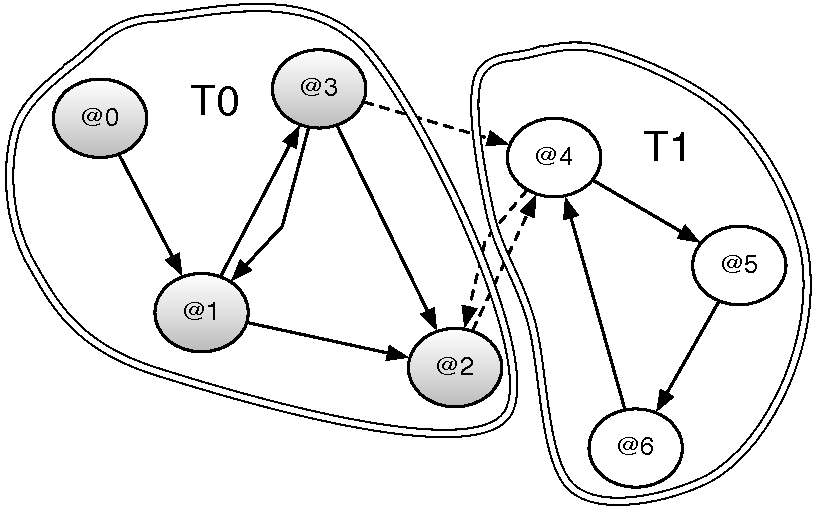
\includegraphics[width=0.5\textwidth]{topologygraph.pdf}}
 \end{center}
    \caption{Partitioning a program with 7 nodes.}
    \label{fig:clustering}
\end{figure}

\subsection{Threads}

The work queue is actually implemented as two queues. First, there's one double-linked list for nodes
without priority called the \emph{normal queue}.
We use a double-linked list because it will be easier to move the node from this queue to the
\emph{priority queue}. The priority queue is an array based binary heap data structure that contains
all the unprocessed nodes with priority. Note that all those data structures are intrusive: all data
fields used in the queues are part of the node data structure such as the \texttt{next} and \texttt{prev}
fields of the normal queue. Each node also contains flags that will tell in which queue they are currently
in and if they have facts to process.

\subsection{Nodes}

%\begin{comment}
\begin{figure}[h!]
     \centering
   \resizebox{7cm}{!}{

    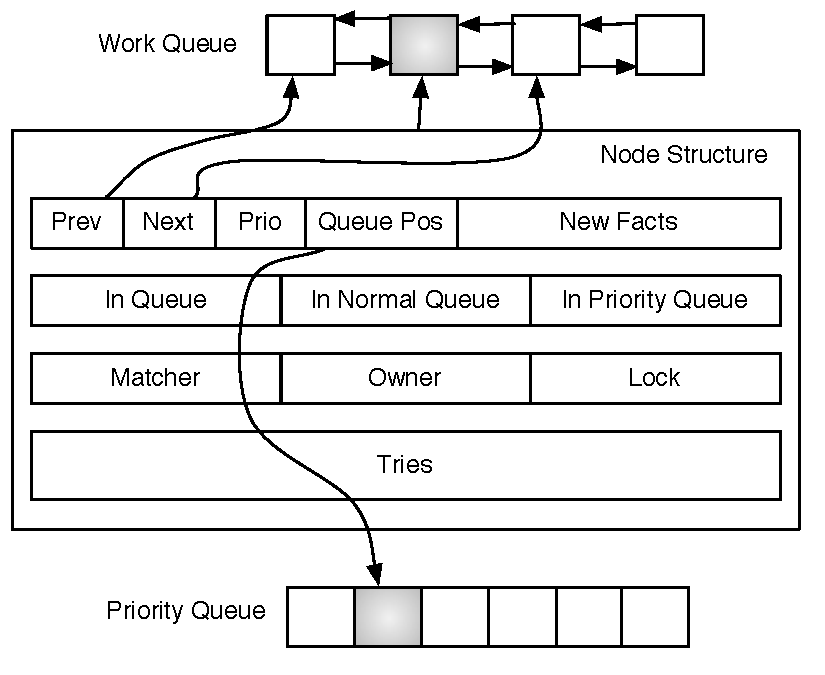
\includegraphics[width=0.5\textwidth]{node.pdf}}
    \caption{The node data structure.}
    \label{fig:node}
\end{figure}
%\end{comment}

In Fig.~\ref{fig:node} we present the node data structure and its fields. We summarize the data below:

\begin{description}
   \item[queue intrusive data]: Includes the field \texttt{Prev} (for the normal queue), \texttt{Next} (for the normal queue), \texttt{Prio} (priority) and \texttt{Queue Pos} (for the priority queue).
   \item[flags]: If the node is currently in the queue and in which queue. Includes \texttt{In Queue}, \texttt{In Normal Queue} and \texttt{In Priority Queue}.
   \item[fact queue]: A simple linked-list containing the unprocessed facts called \texttt{New Facts}.
   \item[database]: All the facts already processed and are true for this node. Is implemented as a trie and it is called \texttt{Tries}.
   \item[rule matcher]: The \texttt{Matcher} maintains the number of facts per predicate and which rules can be activated next. This is used for selecting the candidate rules.
   \item[owner]: Pointer to the owner thread. \texttt{Owner} in the figure.
   \item[lock]: A \texttt{Lock} mutex used to manipulate the node.
\end{description}

\subsection{Work Stealing}

When a thread runs out of nodes to process, it will pick a thread at random and try to steal one node
from the target thread. The stealer thread will pop a node from either the priority queue or the normal queue. We use locks for mutual exclusion when dealing with those queues. Note that when a
node is stolen, its owner information also changes to the stealer thread.

It is important to note that whenever a node sends a coordination action fact to a node in another thread, the fact is ignored, due to the costs of sending
coordination data between threads.

\subsection{Database}

The node database is implemented using the trie data structure. Tries are trees where facts are indexed
by the common prefix. Because we need to delete facts from the database, we implement each trie level
as a double linked list so trie nodes can be easily removed. If a trie level has too many nodes, we
transform the linked list into a hash table in order to improve lookup.

Each node uses a trie per predicate to store facts. During evaluation of rule bodies, we build a
\emph{match object}, which matches some arguments of the target predicate to instantiated values, so
that by searching the predicate trie from top to bottom, we can easily discard invalid trie branches.

\begin{comment}
\subsection{Memory Allocator}

Memory allocation is done using pools of memory objects local to each thread. This reduces contention in
memory allocation.
\end{comment}

\section{Programs}\label{sec:programs}
In this section, we describe how some programs are implemented. We will present a graph algorithm
(single source shortest path), a machine learning algorithm (splash belief propagation) and a logic puzzle (N queens).

\subsection{Shortest Path}

The Single Source Shortest Path (SSSP) is a graph algorithm where we want to compute the
distance of all nodes to a single node. The full code is presented in Fig.~\ref{code:shortest_path_program}.
The graph is represented using the \texttt{edge(A, B, W)} fact, where $A \rightarrow B$ is a directed edge
from node $A$ to $B$ with distance $W$. Note that the axioms are not shown in the code. The second
predicate is \texttt{path(A, D, F)}, where $D$ is the distance of node $A$ to our initial node and $F$
is a flag indicating if this path has been processed (as explained below).

Every node may have several \texttt{path} facts. From this set of facts, the node will select
the path with the least distance (with rule 1 and 2) and then propagate it using the third rule.
When a path is used for propagation, we make sure that the path flag is \texttt{notused}
because we do not want to propagate the same distance twice. When the rule is fired, the flag
then changes to \texttt{used}.

We start with the axiom $\texttt{path(startnode, 0, notused)}$ (the distance to the starting node is 0).
This will kickstart the computation by propagating the initial distance to the neighbor nodes using
rule 3. We also use 2 coordination directives:

\begin{itemize}
   \item \texttt{priority @order asc}: paths are picked in ascending order.
   \item \texttt{set-priority(B, float(D + W))}: to change the node's priority upon the computation of
a new distance.
\end{itemize}

With these directives, we ensure that we pick the node with the smallest path distance
first. If we are only using 1 thread, then our algorithm will behave like the Dijkstra's shortest
path algorithm~\cite{Dijkstra}. When using more than 1 thread, each thread will pick the smallest
path from a subset of nodes. This is the first example where using coordination directives will
improve the speed of execution since we avoid propagating some of the paths.

\begin{figure}[h!]
\small\begin{verbatim}
type route edge(node, node, int).
type linear path(node, int, int).

priority @order asc.

const used = 1.
const notused = 0.

path(startnode, 0, notused).

path(A, B, used), path(A, B, notused) -o path(A, B, used).

path(A, B1, X), path(A, B2, Y), B1 <= B2 -o path(A, B1, X).

path(A, D, notused)
   -o {B, W | !edge(A, B, W) |
         path(B, D + W, notused),
         set-priority(B, float(D + W))},
      path(A, D, used).
\end{verbatim}
  \caption{Shortest Path Program.}
  \label{code:shortest_path_program}
\end{figure}
\normalsize

\subsection{Splash Belief Propagation}

Loopy Belief Propagation~\cite{Murphy99loopybelief} (LBP) is an approximate inference algorithm
used in graphical models with cycles. In its essence LBP is a sum-product message passing algorithm
where nodes exchange messages with their immediate neighbors and apply some computations to the messages
received.

LBP is an algorithm that maps very well to the \lang model. In its original form, we need to compute
the belief of all nodes for several iterations and also synchronize after each iteration.
However, it is still possible to apply
some optimizations in order to take advantage of the fact that LBP will converge even when using
an asynchronous approach. So, instead of computing the belief iteratively,
we first keep track of all messages sent/received (and overwrite them when we receive a new one)
and recompute the belief when we want, instead of synchronizing between nodes.
This way, we can prioritize the computation of beliefs when
a node changes significantly in terms of belief value. When that happens, we set the priority of its
neighbors so that they can recompute their beliefs using important messages.

The asynchronous approach proves to be a nice improvement over the synchronous version. Still, it
is possible to do even better. Gonzalez et al~\cite{Gonzalez+al:aistats09paraml} developed an optimal
algorithm to compute this algorithm by first building a tree and then updating the beliefs of each node twice, first from the leaves to the root and then from the root to the leaves. The root of this tree
is the node with the highest priority (from the changes in belief) while the other nodes in the tree
must have a non-zero priority. Note that the priorities are updated whenever a neighbor updates
their belief. These splash trees are built iteratively until we reach convergence.

The code in Fig.~\ref{code:sbp} presents the coordination component of the Belief Propagation problem.
Please note that we just appended the code in Fig.~\ref{code:sbp} to a working but unoptimized version
of the algorithm.
In the coordination code have three sections:
\begin{description}
   \item[Tree building]: Each node has a \texttt{waiting} fact that is used to start the tree building process. When the highest priority is picked we create the token that will navigate through the tree. Note that in rule 4 we check if the priority of the new node to add to the tree is positive and that both nodes are in the same CPU. We want the tree to be kept in the same CPU.
   \item[First phase]: In the third rule, when we reach a certain number of nodes in the tree, we generate \texttt{first-phase} in order to update the beliefs of all nodes in tree starting from the leaves and ending at the root. As we update the nodes, we generate \texttt{update} to update the belief values.
   \item[Second phase]: In the second phase we go from the root to the leaves and update the beliefs a second time.
\end{description}

When we have several threads, every thread will generate their own trees by taking into account the highest priority node in their own queues. We do not use work stealing for this program because that would interfere with our coordination.

\begin{figure}[h!]
\small\begin{verbatim}
// TREE BUILDING
// continue tree
waiting(A), token(A, All, Next) -o token(A, All, Next).
// start tree
waiting(A), @priority(A, A, P), P > 0.0
   -o token(A, [A], [A]).
// end tree building
token(A, All, Next), length(All) > maxnodes
   -o first-phase(A, All, reverse(All)).
// expand tree
token(A, All, [A | Next])
   -o [collect => L | Side | !edge(A, L, Side),
         0 = count(All, L),
         0 = count(Next, L),
         @priority(A, L, P), P > 0.0,
         @cpu-id(A, L, Id1),
         @cpu-id(A, A, Id2), Id1 = Id2 |
         send-token(A, All, Next ++ L)].

send-token(A, All, [])
   -o first-phase(A, All, reverse(All)).
send-token(A, All, [B | Next])
   -o schedule-next(B),
      token(B, All ++ [B], [B | Next]).

// FIRST PHASE
first-phase(A, [A], [A]) -o second-phase(A, [], A).
first-phase(A, [A, B | Next], [A])
   -o update(A), schedule-next(B),
      second-phase(B, [B | Next], A).
first-phase(A, All, [A, B | Next])
   -o update(A), schedule-next(B),
      first-phase(B, All, [B | Next]).

// SECOND PHASE
second-phase(A, [], _)
   -o set-priority(A, 0.0), waiting(A), update(A).
second-phase(A, [A], Back)
   -o update(A), waiting(Back),
      waiting(A), set-priority(A, 0.0).
second-phase(A, [A, B | Next], Back)
   -o update(A), waiting(Back), schedule-next(B),
      second-phase(B, [B | Next], A).
\end{verbatim}
  \caption{Coordination code for the Splash Belief Propagation.}
  \label{code:sbp}
\end{figure}
\normalsize

%\begin{comment}
\subsection{N Queens}

The N queens~\cite{8queens} puzzle is the problem of placing N chess queens on an NxN chessboard so
that no pair of two queens attack each other. The specific challenge of finding all the distinct
solutions to this problem is a good benchmark in designing parallel algorithms.

We will not show the algorithm in this paper due to the lack of space, but we will explain in general
terms how we solve the problem in \lang. First, we consider each square of the chessboard as a node
that can communicate with the adjacent left, right and bottom squares, but not top square.
The states are represented as a list of integers, where each integer is the column number where
the queen was placed. For example $[2, 0]$ means that a queen was placed in $(0, 0)$ and $(1, 2)$.

An empty state is instantiated in the top-left node and is then propagated to all nodes in the same row.
Every node will then check if a queen can be placed on the square. If true, each node will send the new
state to the row below.
Recursively, when a node receives a new state, it will (1) send the state to the left
and to the right and (2) try to place the queen in its square. With this method,
all states will be computed since we have facts for each valid state
at that point. When a square cannot place a queen, that state is deleted.
When the program ends, the states will be placed in the bottom row.

We find our solution very elegant, since it can be easily executed in parallel and there are no
wasted computations, because any distinct placement will be computed only once.

\begin{comment}
\begin{figure}[h!]
\small\begin{verbatim}
type left(node, node).
type right(node, node).
type down(node, node).
type coord(node, int, int).
type linear propagate-left(node, list node, list int).
type linear propagate-right(node, list node, list int).
type linear receive-down(node, list node, list int).
type linear test-and-send-down(node, list node, list int).
type linear test-y(node, int, list int, list node, list int).
type linear test-diag-left(node, int, int, list int, list node, list int).
type linear test-diag-right(node, int, int, list int, list node, list int).
type linear send-down(node, list node, list int).
type linear final-state(node, list node, list int).

const size = 11.

receive-down(@0, [], []).

receive-down(A, Nodes, Coords)
   -o {R | !right(A, R), R <> A | propagate-right(R, Nodes, Coords)},
      {L | !left(A, L), L <> A | propagate-left(L, Nodes, Coords)},
      test-and-send-down(A, Nodes, Coords).

propagate-left(A, Nodes, Coords)
   -o {L | !left(A, L), L <> A | propagate-left(L, Nodes, Coords)},
      test-and-send-down(A, Nodes, Coords).

propagate-right(A, Nodes, Coords)
   -o {R | !right(A, R), R <> A | propagate-right(R, Nodes, Coords)},
      test-and-send-down(A, Nodes, Coords).

test-and-send-down(A, Nodes, Coords),
!coord(A, X, Y)
   -o test-y(A, Y, Coords, Nodes, Coords).

test-y(A, Y, [], Nodes, Coords), !coord(A, OX, OY) -o test-diag-left(A, OX - 1, OY - 1, Coords, Nodes, Coords).
test-y(A, Y, [X, Y1 | RestCoords], Nodes, Coords), Y = Y1 -o 1. // fail
test-y(A, Y, [X, Y1 | RestCoords], Nodes, Coords), Y <> Y1 -o test-y(A, Y, RestCoords, Nodes, Coords).

test-diag-left(A, X, Y, _, Nodes, Coords),
X < 0 || Y < 0,
!coord(A, OX, OY)
   -o test-diag-right(A, OX - 1, OY + 1, Coords, Nodes, Coords).

test-diag-left(A, X, Y, [X1, Y1 | RestCoords], Nodes, Coords),
X = X1, Y = Y1
   -o 1. // fail

test-diag-left(A, X, Y, [X1, Y1 | RestCoords], Nodes, Coords),
X <> X1 || Y <> Y1
   -o test-diag-left(A, X - 1, Y - 1, RestCoords, Nodes, Coords).

test-diag-right(A, X, Y, [], Nodes, Coords),
X < 0 || Y >= size,
!coord(A, OX, OY)
   -o send-down(A, [A | Nodes], [OX, OY | Coords]).

test-diag-right(A, X, Y, [X1, Y1 | RestCoords], Nodes, Coords),
X = X1, Y = Y1
   -o 1. // fail

test-diag-right(A, X, Y, [X1, Y1 | RestCoords], Nodes, Coords),
X <> X1 || Y <> Y1
   -o test-diag-right(A, X - 1, Y + 1, RestCoords, Nodes, Coords).

send-down(A, Nodes, Coords),
!down(A, A)
   -o final-state(A, Nodes, Coords).
   
send-down(A, Nodes, Coords),
!down(A, B),
A <> B
   -o receive-down(B, Nodes, Coords).
\end{verbatim}
  \caption{Visit program.}
  \label{code:visit}
\end{figure}
\normalsize
%\end{comment}
\end{comment}

\section{Experiments}
With our experiments we want to show three key results. The first result is that our virtual machine performs well when running multiple threads,
i.e., it can reasonably schedule the execution of programs to reduce execution time and increase parallel speedup. The second result is that by using coordination directives, programs perform faster. Third, we want to show that our programs are usually shorter than programs written in other languages.  

In our experimental setup, we used a machine with
four AMD Six-Core Opteron TM 8425 HE (2100 MHz) chips (24 cores) and 64 GB of DDR-2 667MHz (16x4GB) RAM,
     running GNU/Linux (kernel 2.6.31.5-127 64 bits).
     We compiled our virtual machine using GCC 4.4.5 (g++) with the flags \texttt{-O3 -std=c+0x -march=x86-64}.
     We run all experiments 3 times with the same configuration and then we averaged the run time.

\subsection{Parallel Experiments}

For the parallel results, we run each program using 1, 2, 4, 6, 8, 10, 12, 14 and 16 threads and compared the runtime against the execution of the sequential version of the virtual machine. We used the following programs:

\begin{description}
   \item[greedy graph coloring]: In this program, we attempt to color each node of a graph so that no two adjacent nodes have the same color. We start with 15 colors and expand the number of colors when we cannot color the graph.
   \item[pagerank]: The asynchronous PageRank algorithm without synchronization between iterations. Every time a node sends a new rank to its neighbors and the change was significant, the neighbors are scheduled to recompute their ranks.
   \item[N queens]: Already explained before. We use an 11x11 board.
\end{description}

In Fig.~\ref{exp:graph_coloring} we present the speedup results for the graph coloring program. In the first plot, we show the speedup for a graph of 12000 webpages. Since this dataset follows the power law, that is, there is a small number of pages with a lots of links (1\% of the nodes have 75\% of the edges), the speedup is not as good as the one shown when using a random dataset of 2000 nodes, where each node has more or less the same number of links. In the weather web graph 20\% of the nodes have 75\% of the edges, much less than the search engine dataset, and it shows in the results.

\newcommand{\figsize}[0]{4.5cm}

\begin{figure*}[htp]
   \centering
   \resizebox{\figsize}{!}{\subfigure[Using a search engine web graph (almost 12000 nodes)]{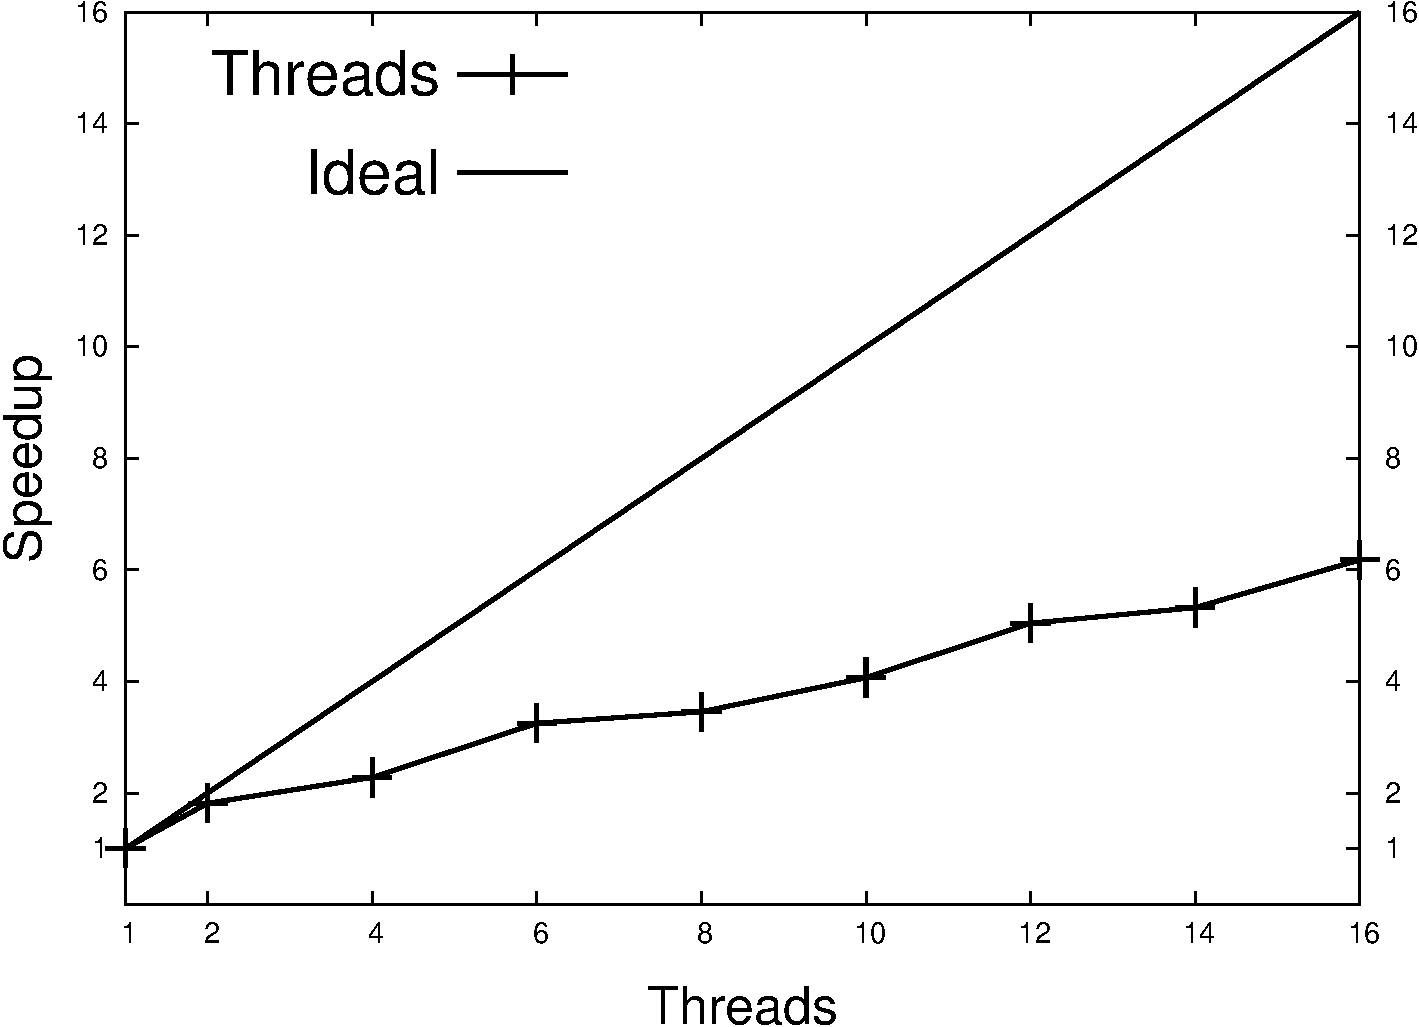
\includegraphics[width=0.5\textwidth]{speedup_greedy-graph-coloring-search_engines.pdf}}}
   \resizebox{\figsize}{!}{\subfigure[Using a weather web graph (around 8000 nodes)]{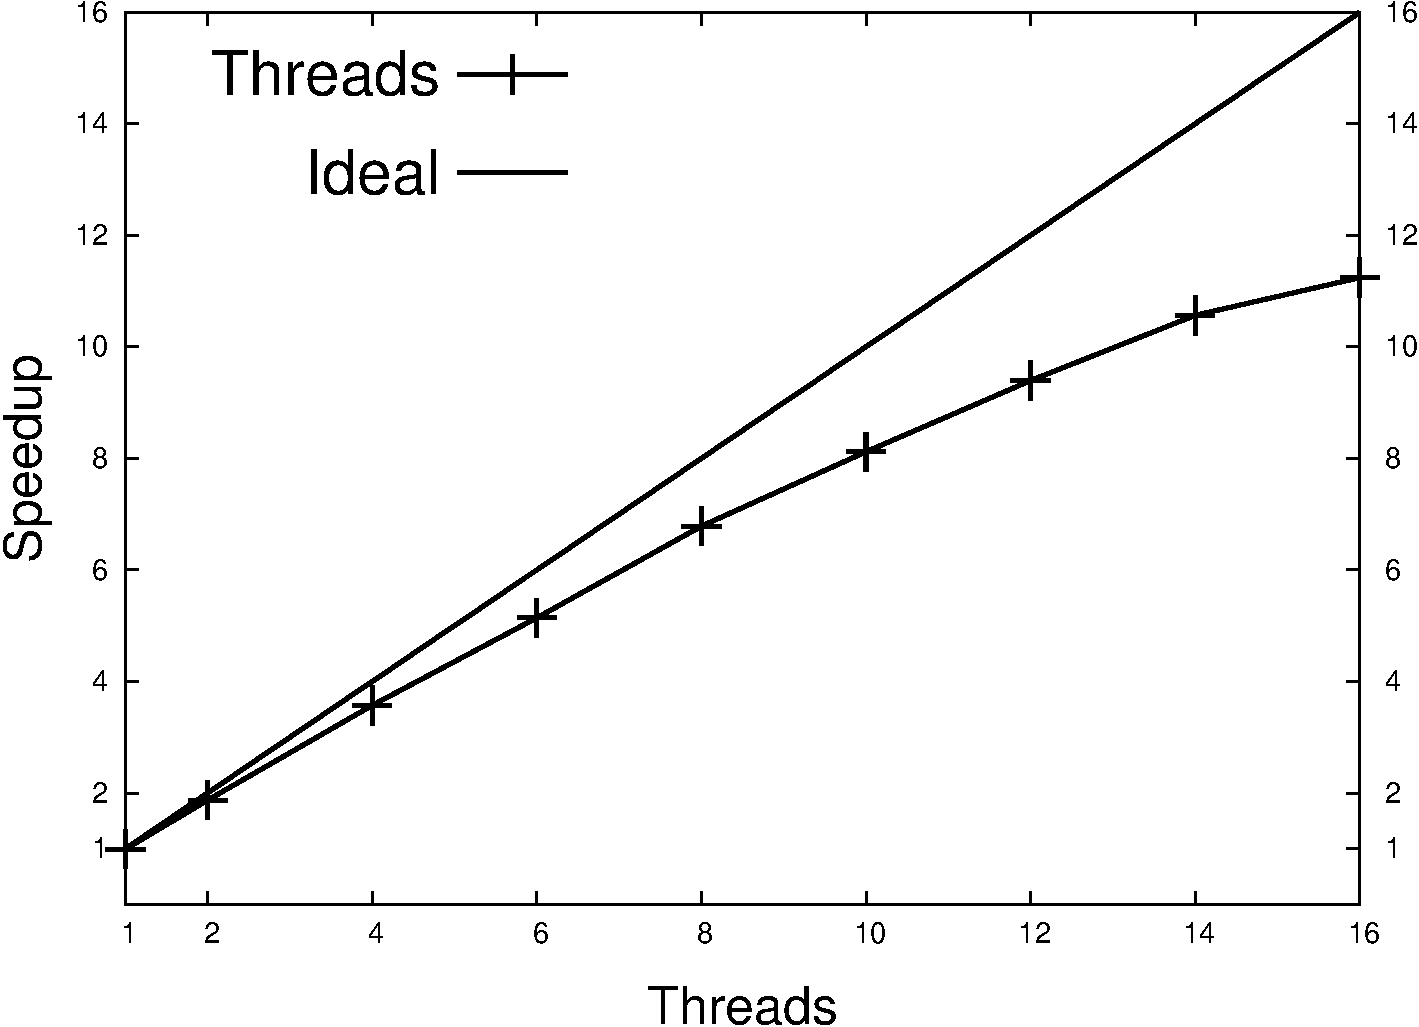
\includegraphics[width=0.5\textwidth]{speedup_greedy-graph-coloring-weather.pdf}}}
   \resizebox{\figsize}{!}{\subfigure[Using a random graph (with 2000 nodes)]{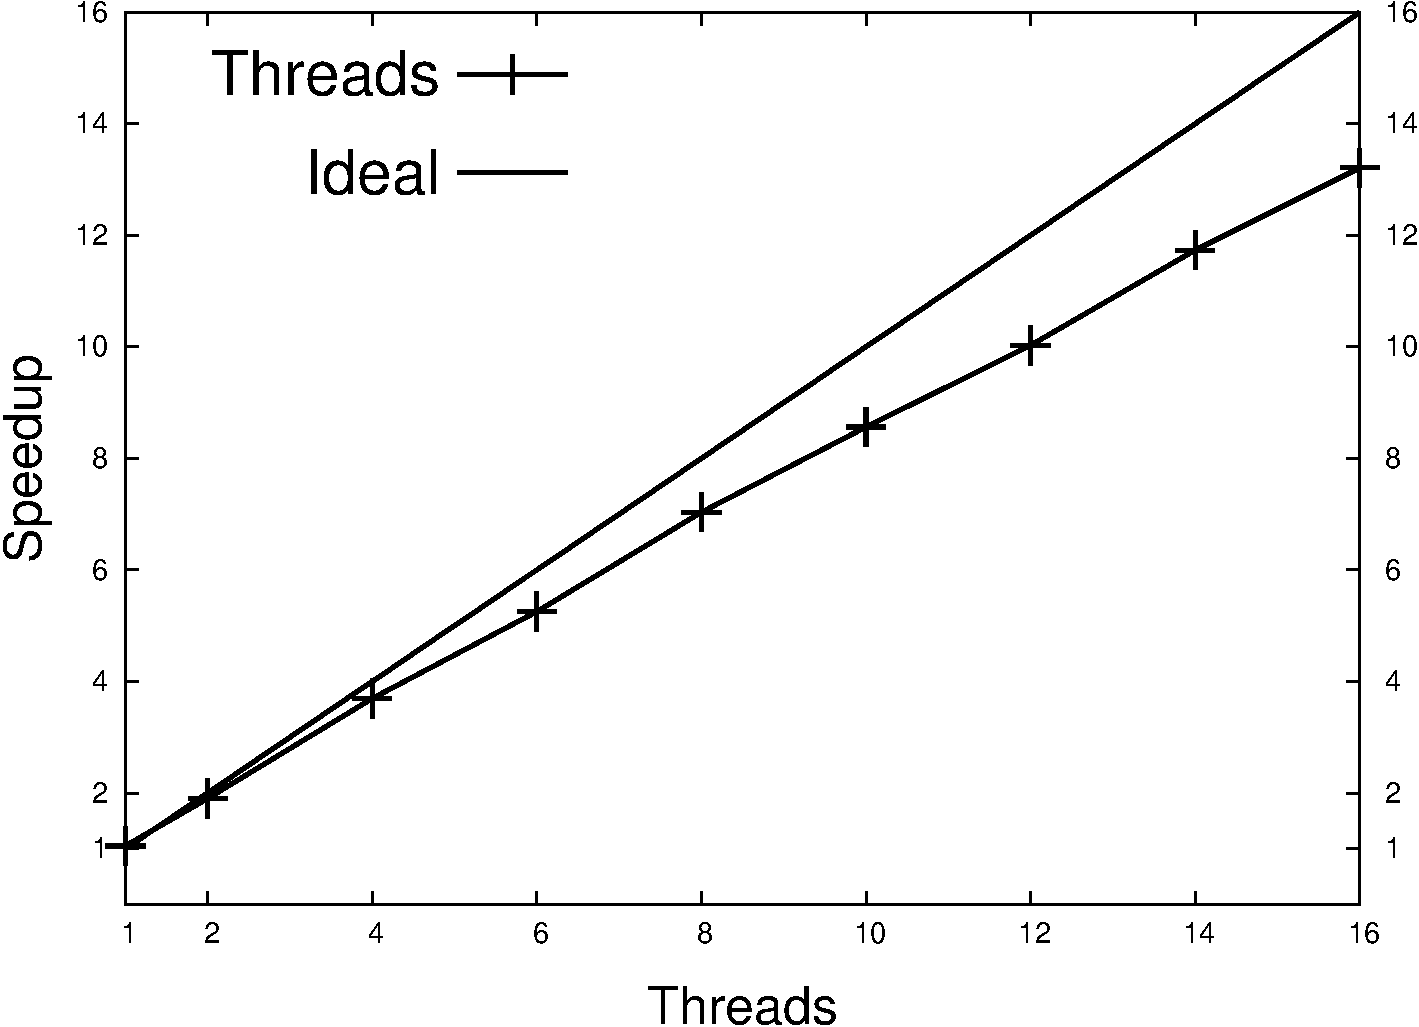
\includegraphics[width=0.5\textwidth]{speedup_greedy-graph-coloring-2000.pdf}}}
   \caption{Experimental results for the greedy graph coloring algorithm.}
   \label{exp:graph_coloring}
\end{figure*}

\begin{figure*}[htp]
   \centering
   \resizebox{\figsize}{!}{\subfigure[Using a search engine web graph (almost 12000 nodes)]{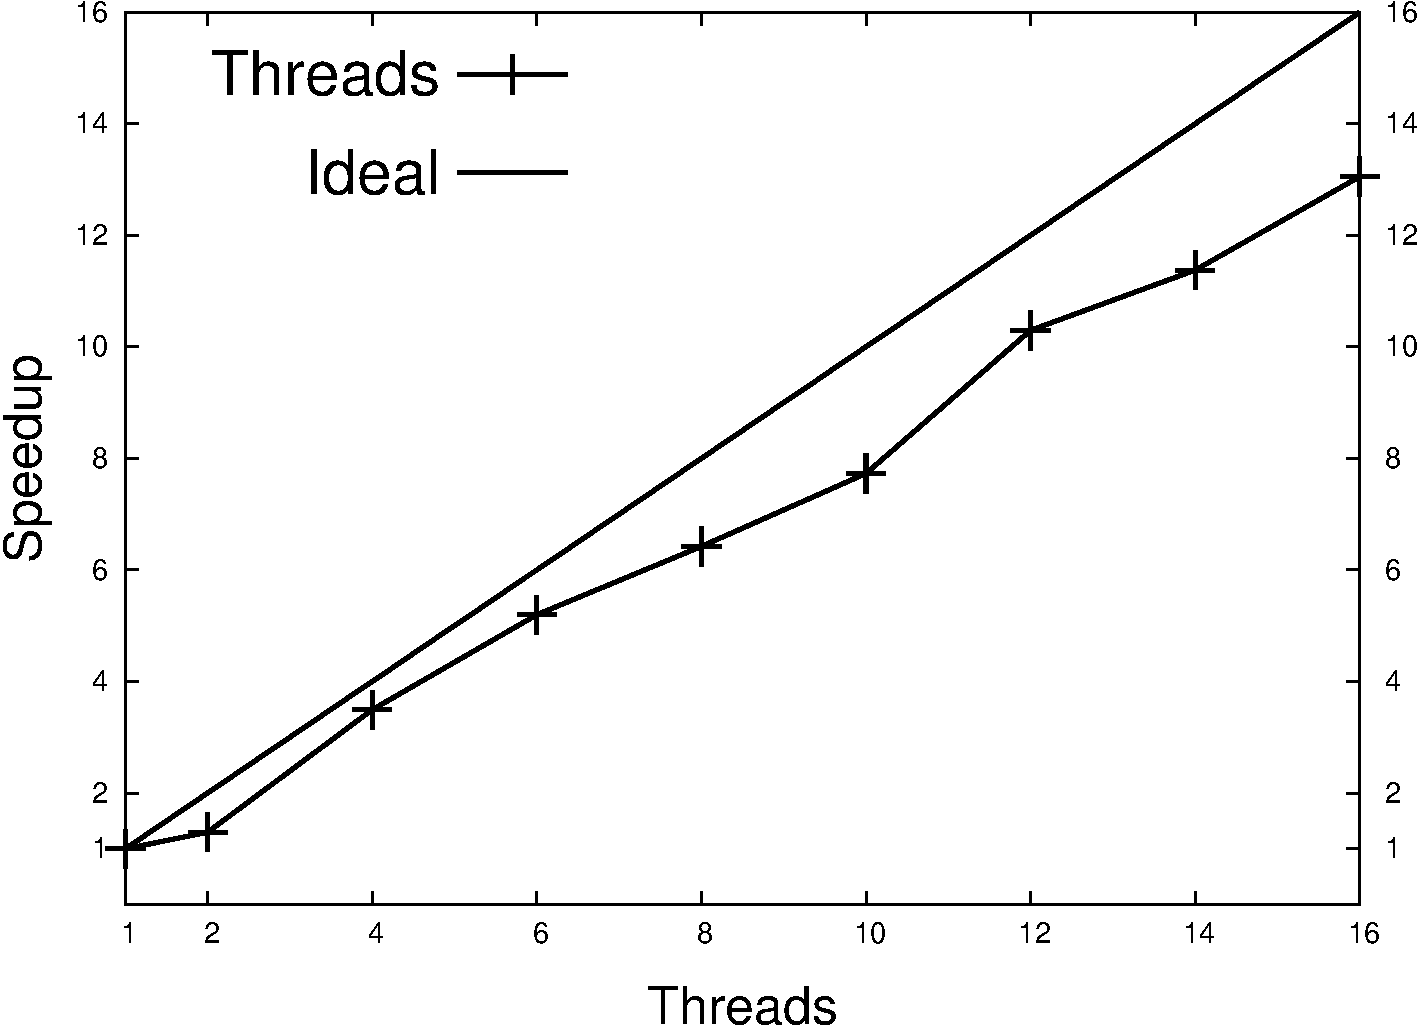
\includegraphics[width=0.5\textwidth]{speedup_pagerank-search_engines.pdf}}}
   \resizebox{\figsize}{!}{\subfigure[Using a movie web graph (almost 8000 nodes)]{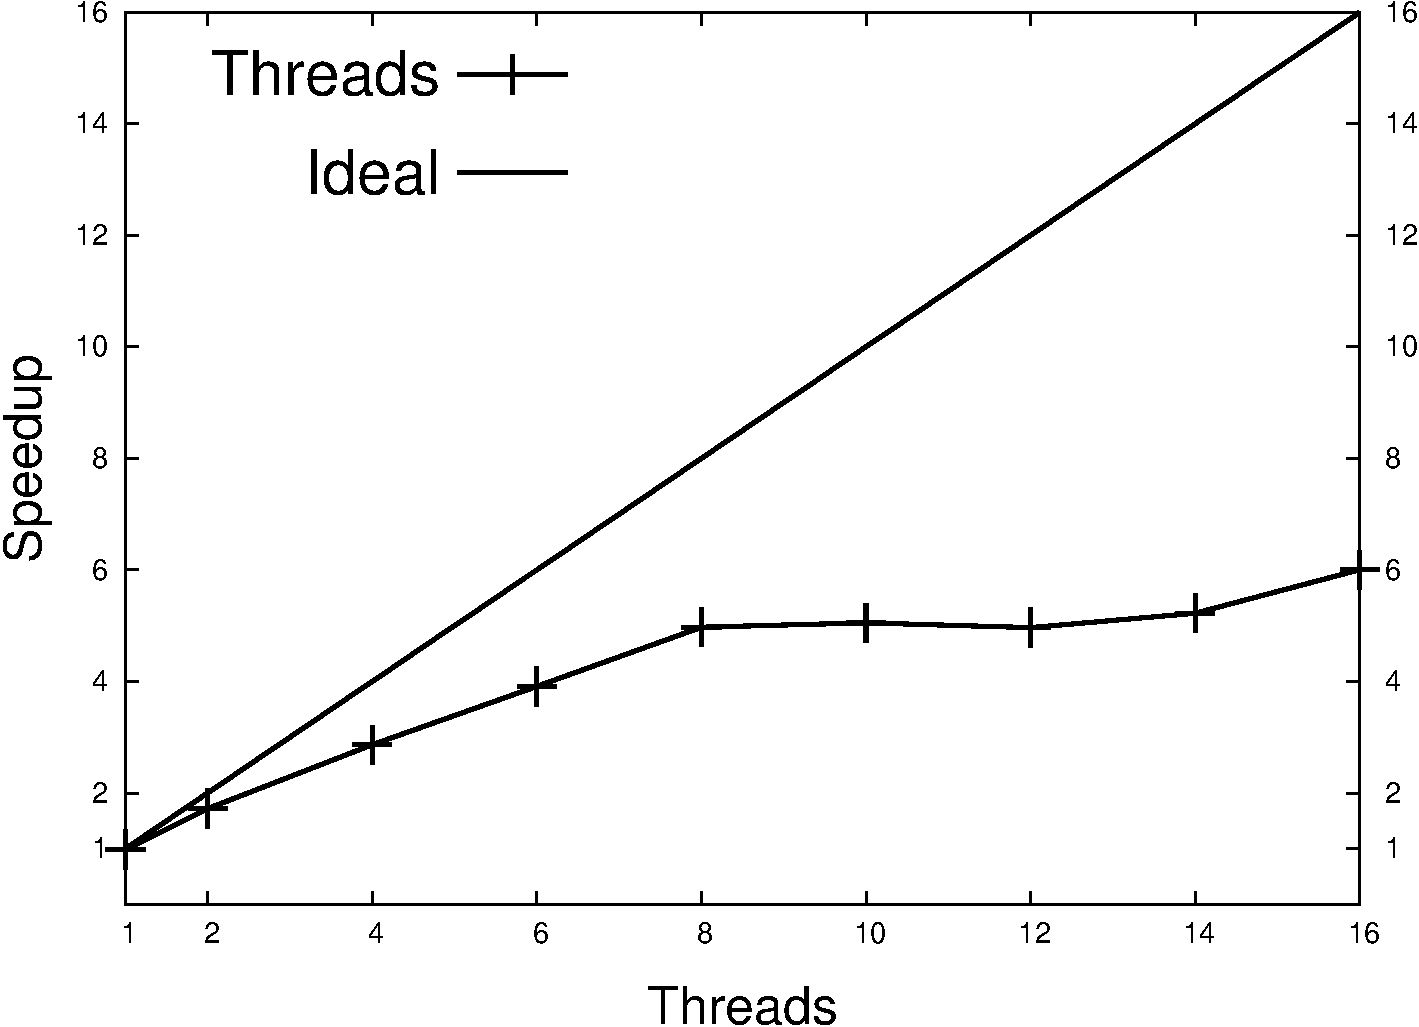
\includegraphics[width=0.5\textwidth]{speedup_pagerank-movies.pdf}}}
   \resizebox{\figsize}{!}{\subfigure[Using a random, dense graph (500 nodes)]{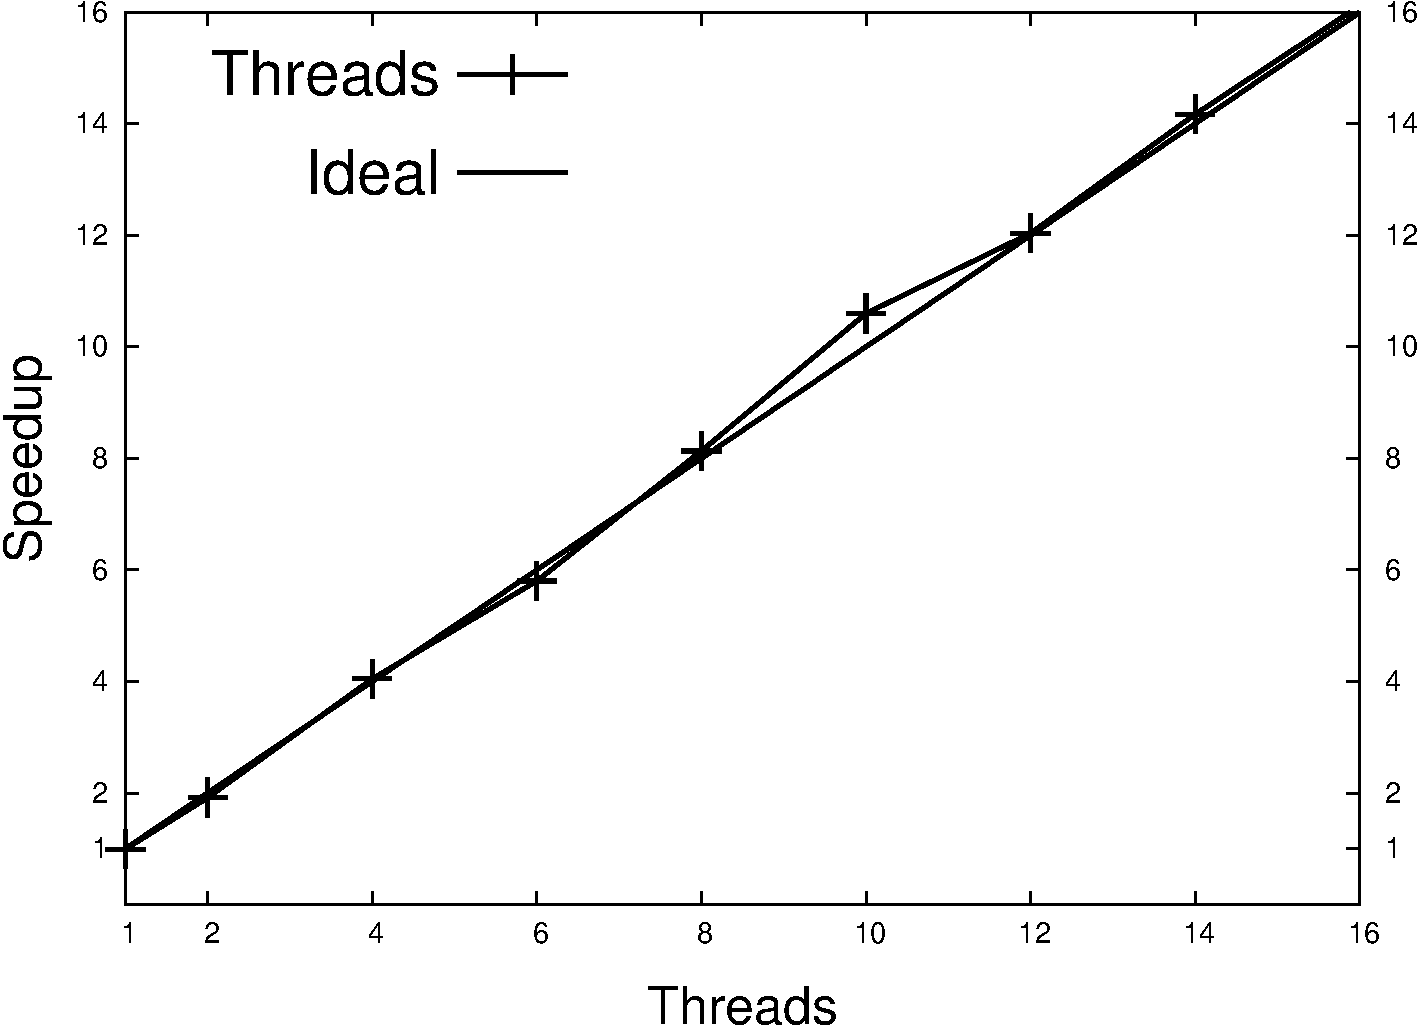
\includegraphics[width=0.5\textwidth]{speedup_pagerank-500.pdf}}}
   \caption{Experimental results for the asynchronous PageRank algorithm.}
   \label{exp:pagerank}
\end{figure*}

The PageRank results are shown in Fig.~\ref{exp:pagerank}. We have used the same web graph dataset as before and a new dataset representing movie websites \footnote{Both the search engine and movie web graphs were retrieved from \url{http://www.cs.toronto.edu/~tsap/experiments/download/download.html}}. We notice that the search engine graph dataset is big enough to allow good execution improvements even with 16 threads, while the movie graph, being smaller, shows some scaling problems as the number of threads increases. Even though the web graph follows the power law it does not slowdown execution (it happened in the graph coloring algorithm).
For the third plot, we used a random graph with about 500 nodes and 75000 edges. Since the graph is so dense, the runtime is capable of exploiting the
available parallelism, resulting in linear scalability.

\begin{figure}[h!]
     \centering
   \resizebox{\figsize}{!}{

    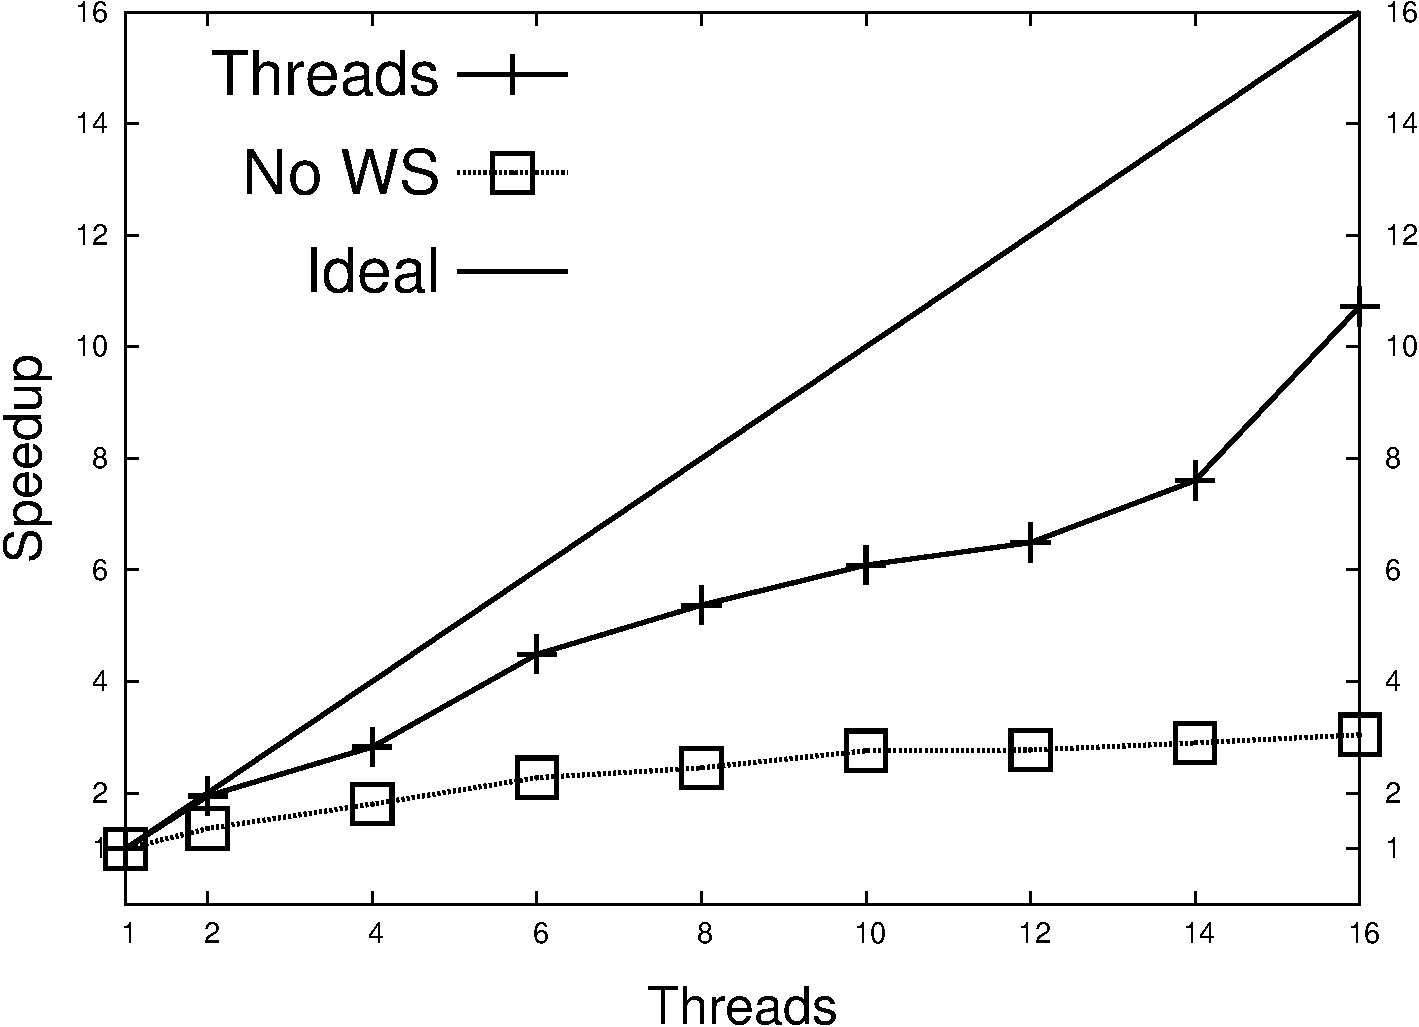
\includegraphics[width=0.5\textwidth]{speedup_8queens-11.pdf}}
    \caption{Experimental results for the N queens program (11x11~board).}
    \label{exp:8queens}
\end{figure}

The results for the N queens program are shown in Fig.~\ref{exp:8queens}. This program is much less regular than the other two, since computation starts at the top of the grid and then rolls down, until only the last row is doing computation. Note that as the computation goes from row to row, the number of states increase, creating even more imbalances. This shows that our system is able to scale well with more traditional algorithms such as N Queens.

\subsection{Coordination Experiments}

In our coordination experiments, we are interested in showing that coordination improves the execution time of programs.
To do this, we are using the following 3 programs:

\begin{description}
   \item[heat transfer]: In the heat transfer program, we have a grid of cells that transfer heat with the neighbor cells by taking into account the edge weights. We use a dataset with a square of cells in the center of the grid with very high heat, while the outer cells have low heat. We use coordination to prioritize the neighbors of cells where rapid heat changes happen.
   \item[shortest path]: We use the SSSP program shown earlier but we extended it to compute the distance to several nodes in order to increase the amount of computation.
   \item[belief propagation]: This is the program explained in the programs section. We build splash trees to improve performance.
\end{description}

Fig.~\ref{exp:heat-transfer} shows the results for the heat transfer program. \textbf{Threads} represents the speedup of the multicore execution
without coordination, while \textbf{Coord} represents the speedup when using coordination directives.
Both execution modes were compared against the sequential execution without coordination.
When using 1 thread, the coordinated version is almost 2 times
faster, however this speedup is slightly reduced as more threads are added. This happens because the \textbf{add-priority} action fact is ignored
when it is sent to a node located in a different thread.
Also note how the \textbf{Coord} line goes over the \textbf{Ideal} line, to the point where using 2 threads is 4 times faster than the sequential
version without priorities.

\begin{figure}[h!]
     \centering
   \resizebox{\figsize}{!}{
   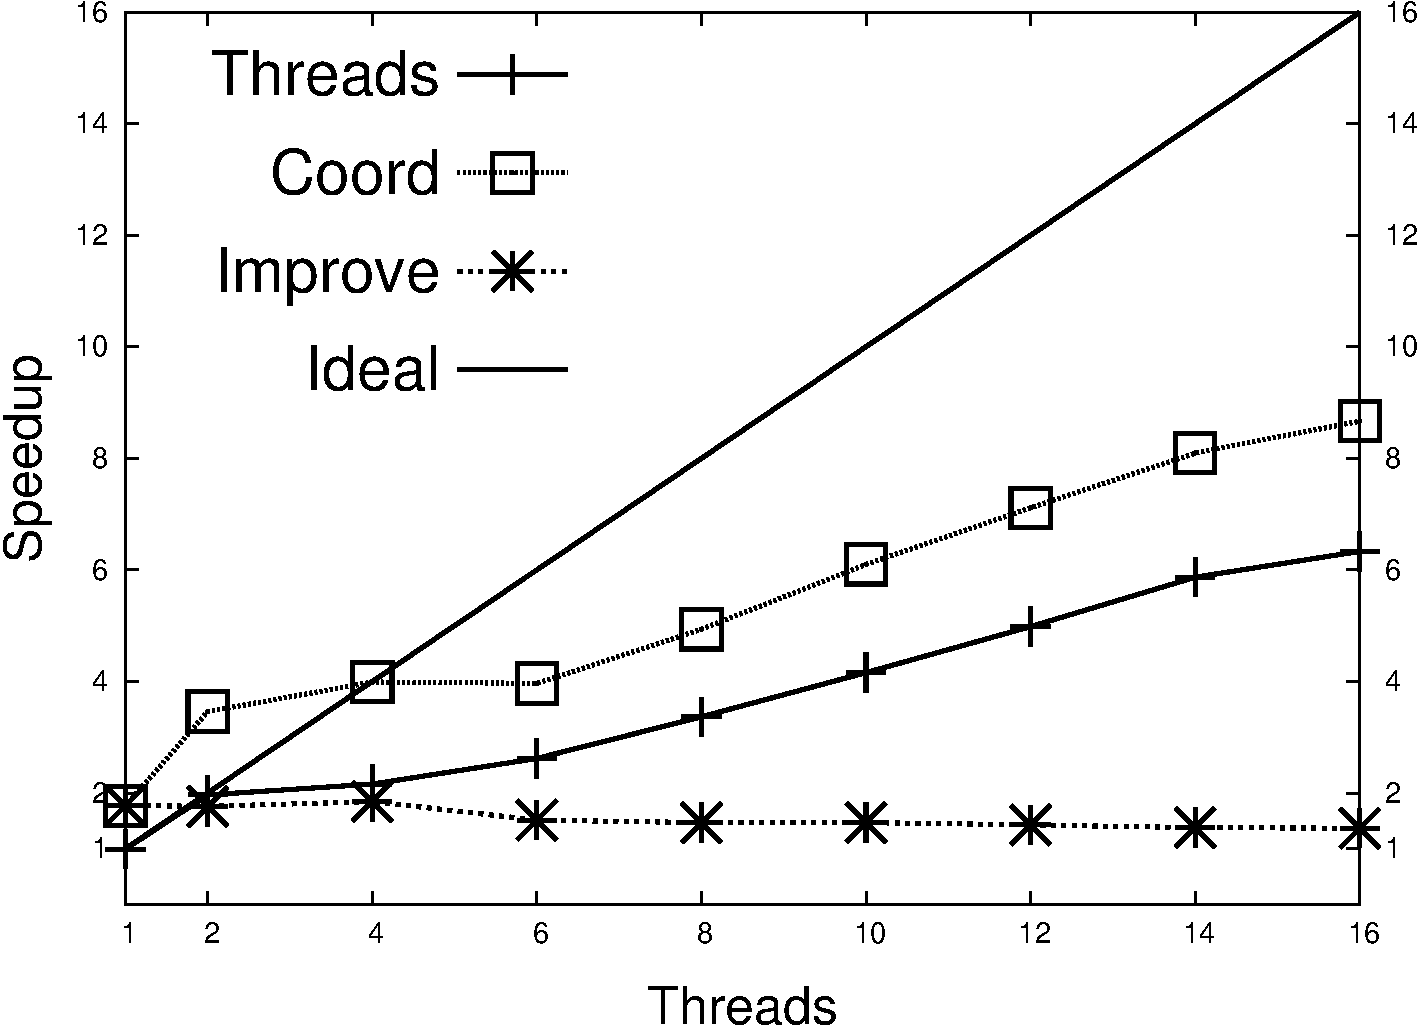
\includegraphics[width=0.5\textwidth]{speedup_heat-transfer-80.pdf}}
   \caption{Experimental results for the heat transfer program.}
   \label{exp:heat-transfer}
\end{figure}

To measure the performance of the SSSP program we used several datasets retrieved from \url{http://toreopsahl.com/datasets}. We computed several
statistics about each dataset, including: the number of nodes (\textbf{\# Nodes}), the number of edges (\textbf{\# Edges}) and
the average number of edges per node (\textbf{Edges / Node}). We also sorted the nodes by number of edges and counted the top number of nodes
with 25\% (\textbf{25\% Edges}), 50\% (\textbf{50\% Edges}) and 75\% (\textbf{75\% Edges}) of all edges.
These statistics and the speedup (\textbf{Speedup}) when using the coordinated version with 1 thread are presented in Table~\ref{tbl:shortest_path_speedup}.

We have tried to understand if there is a correlation between the graph structure and the coordination speedup. We can see that a higher number
of nodes and edges tends to improve execution. The US Airports dataset stands out because it is a small sized graph where a subset of airports
(70) have most connections. The other smaller datasets have a much stable distribution.
Still, the coordinated execution for most datasets is 30\% faster than the regular execution. We also included the speedup plot of the coordinated version
for the US Power Grid dataset in Fig.~\ref{exp:sssp-uspowergrid} that compares against the sequential execution without coordination.

\begin{table*}[ht]

\begin{center}
    \begin{tabular}{| l | c | c | c | c | c | c | c |}
    \hline
    \textbf{Dataset} & \textbf{Speedup} & \textbf{\# Nodes} & \textbf{\# Edges} & \textbf{Edges / Node} & \textbf{25\% Edges} & \textbf{50\% Edges} & \textbf{75\% Edges} \\ \hline \hline
    500 US Airports & 1.497 & 500 & 5960 & 11.92 & 14 & 37 & 70 \\ \hline
    US Power Grid & 1.459 & 4941 & 13188 & 2.67 & 485 & 1374 & 2131 \\ \hline
    Celegans Neural Network & 1.074 & 297 & 2345 & 7.89 & 24 & 65 & 104 \\ \hline
    Facebook like social network & 1.570 & 1899 & 20296 & 10.68 & 42 & 150 & 273 \\ \hline
    Intra-organizational network & 1.090 & 77 & 2288 & 28.94 & 9 & 24 & 36 \\ \hline
    \end{tabular}
\end{center}
     \caption{Summarized information about the datasets used in the SSSP program.}
     \label{tbl:shortest_path_speedup}
\end{table*}

\begin{figure}[h!]
     \centering
   \resizebox{\figsize}{!}{
   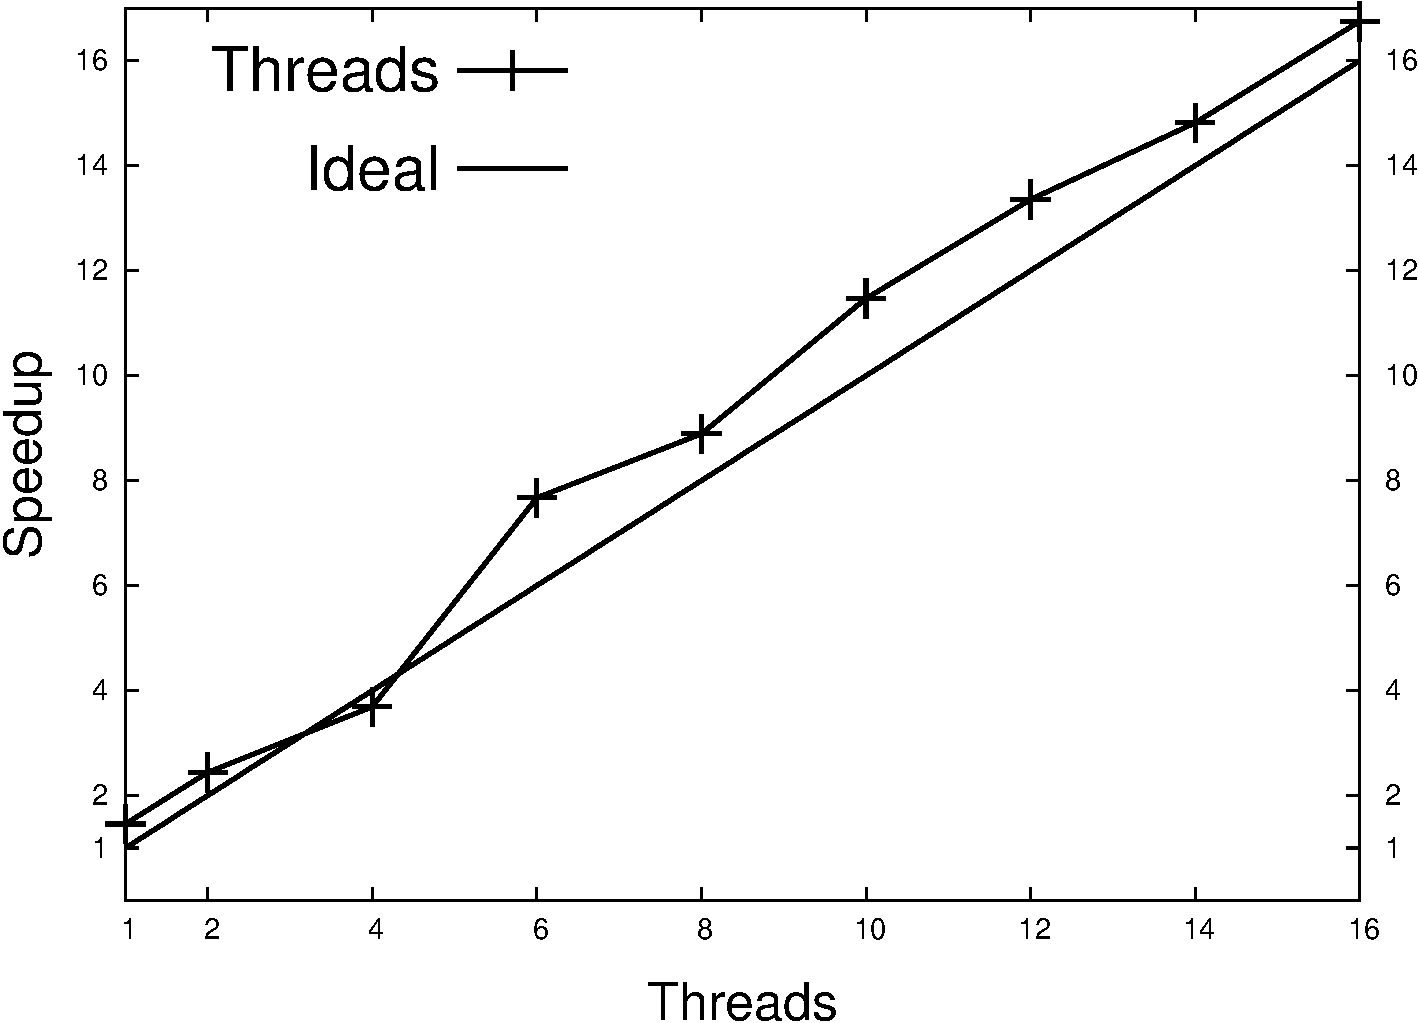
\includegraphics[width=0.5\textwidth]{speedup_uspowergrid.pdf}}
   \caption{Experimental results for the SSSP program with the US Power Grid dataset when using coordination.}
   \label{exp:sssp-uspowergrid}
\end{figure}

While the previous results were computed using only one thread, we also see good speedups with multiple threads. However, the gains reduce as we add
more threads because the decision of picking the best path is done at the thread level, thus reducing the opportunities for optimization.

For the belief propagation (BP) program, we have a noisy image made of 400x400 pixels that needs to be denoised.
To put our implementation to the test, we have also run the GraphLab (version 1) implementation of the same problem. The results are shown
in Fig.~\ref{exp:splashbp}. The first plot presents the scalability results for the simple belief propagation problem. The GraphLab version
uses the \textbf{fifo} scheduler that works identically to the basic \lang scheduler. While both versions show the same scalability pattern,
\lang runs about 3 to 4 times slower since it runs in a virtual machine, where GraphLab runs as a compiled C++ program.

\begin{figure*}[ht]
   \centering
   \resizebox{15cm}{!}{
   \subfigure[Scalability of basic belief propagation.]{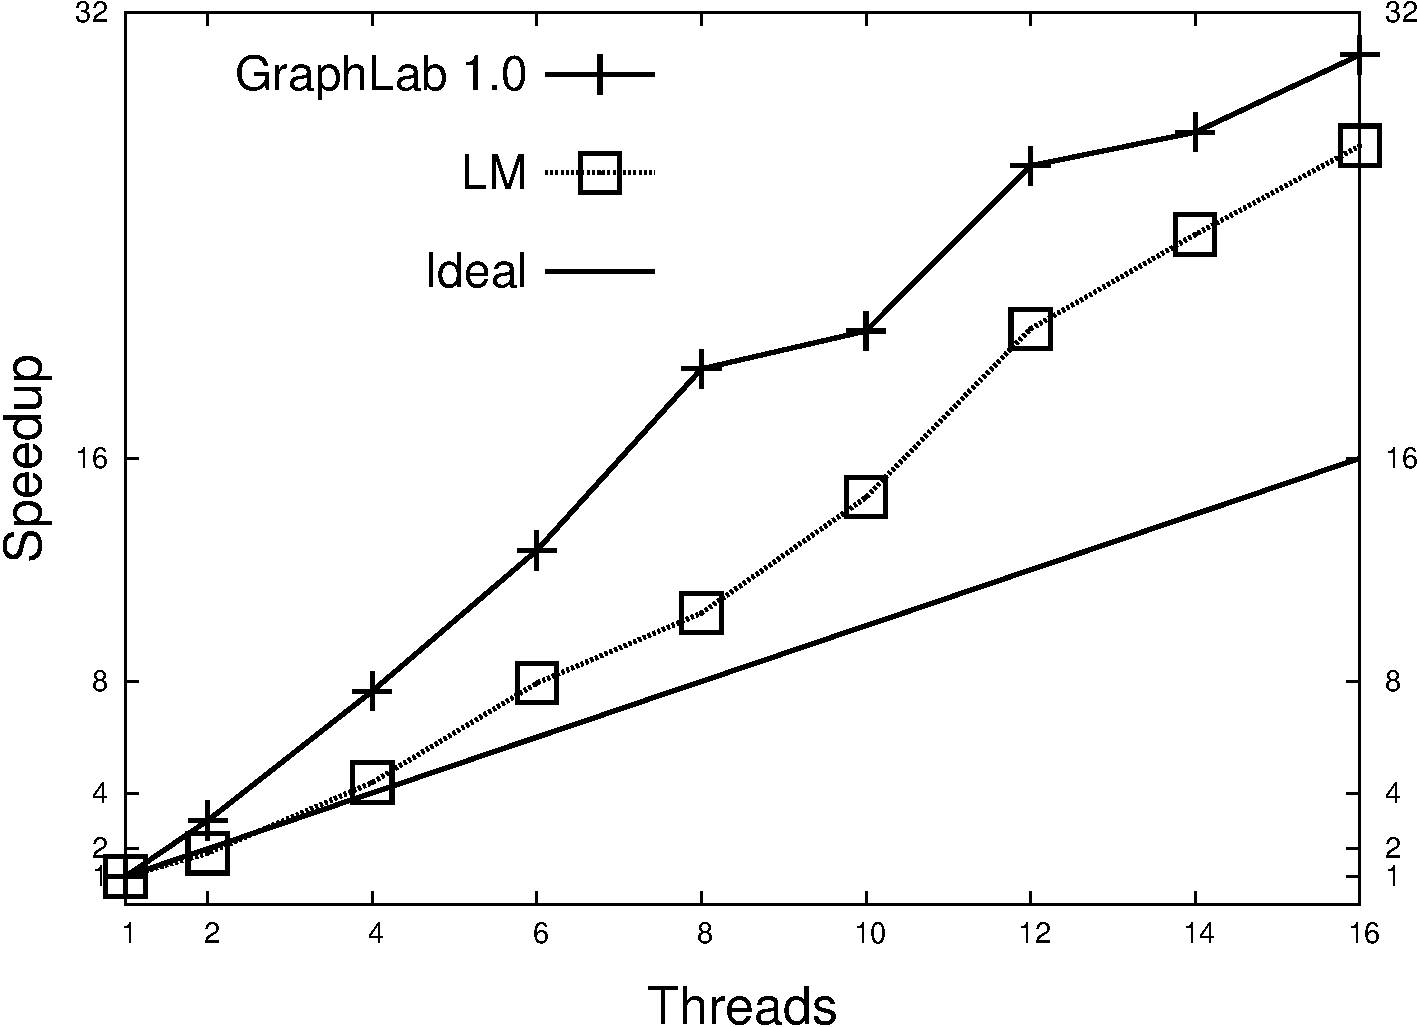
\includegraphics[width=0.7\textwidth]{splash-bp-speedup1_csv.pdf}}
   \subfigure[Scalability of belief propagation with splashes.]{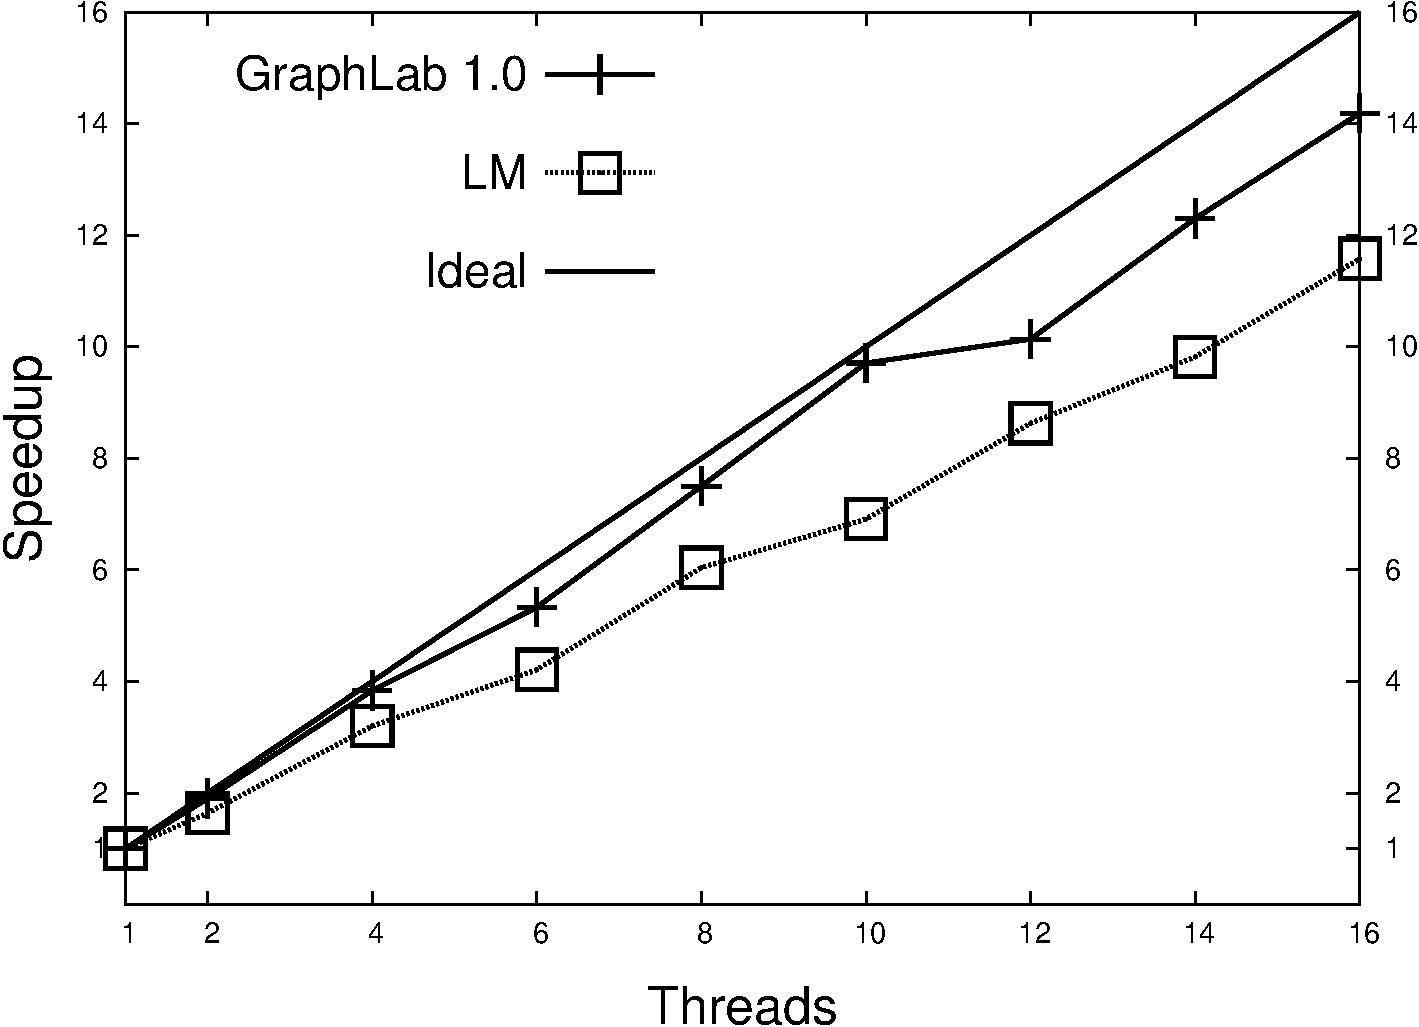
\includegraphics[width=0.7\textwidth]{splash-bp-speedup2_csv.pdf}}
   \subfigure[Coordination improvements by using splashes.]{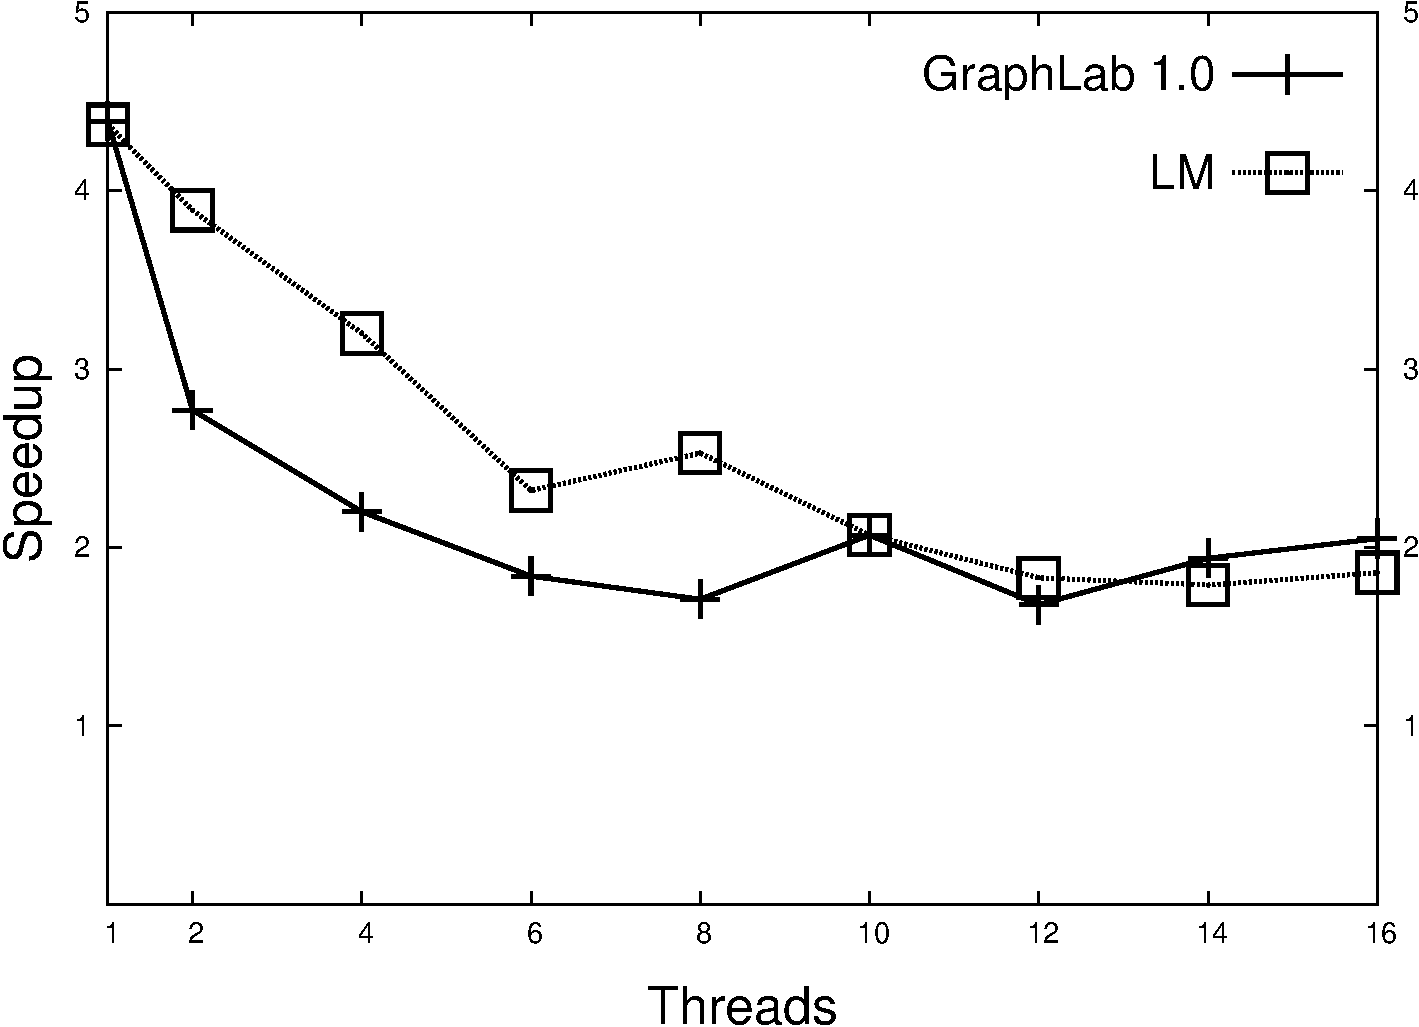
\includegraphics[width=0.7\textwidth]{splash-bp-improv_csv.pdf}}}
   \caption{Experimental results for belief propagation with coordination using splashes. The dataset is a 400x400 image.}
   \label{exp:splashbp}
\end{figure*}

The plot in Fig.~\ref{exp:splashbp}~(b) shows the scalability of the coordinated version. For GraphLab we used the \textbf{splash} scheduler, while \lang
runs with the extra coordination rules. Again, the scalability lines are very similar, but GraphLab appears to be slightly more scalable.
Finally, the last plot (Fig.~\ref{exp:splashbp}~(c)) presents the improvements of the coordinated version over the basic version when using a different
number of threads. With only 1 thread, we get almost a 5-fold speedup over the version without coordination. We can also see that adding more threads tends to reduce the effectiveness of splash trees in both systems.

The previous results validate our thesis that applying algorithm dependent scheduling strategies will make execution faster. By using a small set
of action facts and derivation rules we were able to implement complex scheduling strategies present in GraphLab, a practical and powerful machine learning
framework.

\subsection{Memory footprint}

In Fig.~\ref{tbl:memory} we present statistics for the memory footprint of the virtual machine. The data was taken right after the computation was completed
and it represents the memory allocated at that point, including facts and other auxiliary data structures.

\begin{table}[ht]
\begin{center}
      \resizebox{8.5cm}{!}{
    \begin{tabular}{| l | c | c | c | c | }
    \hline
    \textbf{Program} & \textbf{\# Nodes} & \textbf{\# Facts} & \textbf{Memory (MB)} & \textbf{Average (KB)} \\ \hline \hline
    N Queens & 121 & 3164 & 12.13 MB & 102.62 KB \\ \hline
    G. Graph Coloring web & 11659 & 1179671 & 293.06 MB & 25.74 KB \\ \hline
    %G. Graph Coloring weather & 8011 & 144927 & 43.78 MB & 5.60 KB \\ \hline
    PageRank web & 11659 & 1215580 & 309.78 MB & 27.20 KB \\ \hline
    %PageRank movie & 7967 & 147124 & 51.17 MB \\ \hline
    Heat transfer & 6400 & 44480 & 55.82 MB & 8.93 KB \\ \hline
    SSSP US Airports & 500 & 55960 & 16.87 MB & 34.54 KB \\ \hline
    %SSSP US Power Grid & 4941 & 502347 & 159.27 MB \\ \hline
    %BP & 160000 & 2395200 & 4408.48 MB \\ \hline
    Splash BP & 160000 & 2555200 & 2540.96 MB & 16.26 KB \\ \hline
    \end{tabular}}
\end{center}
     \caption{Memory usage of programs.}
     \label{tbl:memory}
\end{table}

In the \textbf{Average (KB)} column, we included the average memory used by a node computed by computing \textbf{Memory (MB)} / \textbf{\# Nodes}.
We note that, for the N Queens program, the average memory is quite high due the number of solutions (2680).
Surprisingly, the Splash BP program shows a low average memory usage even when taking into account the high number of lists used by the program
to store the belief values. In the future, we intend to bring these numbers down by optimizing the code, better fact storage and more efficient
data structures.

\subsection{Language expressiveness and conciseness}

We are also interested in measuring how long \lang programs are when compared to implementations of the same programs in other languages.
We want to show that \lang programs are more concise and can also be run in parallel from the start.

In table~\ref{tbl:length} we show how \lang programs against programs written in other languages in
terms of size. SSSP and the C version of N Queens~\cite{8queens-parallel} are sequential implementations and are difficult
to adapt to run in parallel. Even so, \lang programs are much smaller and in our opinion, easier
to understand. For the N Queens problem, we also included an MPI implementation written in C~\cite{Rolfe:2008:SMA:1473195.1473217}
that is around 10 times longer than the \lang version. We are currently developing an MPI version
of the \lang runtime and preliminary results show some good speedups for this program.

\begin{table}[ht]
\begin{center}
   \resizebox{8.5cm}{!}{
    \begin{tabular}{| c | c | l | c |}
    \hline
    \textbf{Program} & \textbf{\lang} & \textbf{Others} & \textbf{Average} \\ \hline \hline
    SSSP & 6 & 25 (C++) & 24\% \\ \hline
    PageRank & 30 & 60 (GraphLab) & 50\% \\ \hline
    BP & 50 & 90 (GraphLab) & 55\% \\ \hline
    Splash BP & 50 & 350 (GraphLab) & 14\% \\ \hline
    N Queens & 40 & 300 (C~\cite{8queens-parallel}), 400 (MPI~\cite{Rolfe:2008:SMA:1473195.1473217}) & 11\% \\ \hline
    \end{tabular}}
\end{center}
     \caption{Comparison of source code size against other languages.}
     \label{tbl:length}
\end{table}

The GraphLab versions of PageRank, BP and Splash BP are all written in C++ and can be run in
parallel. We only counted the bare minimum number of lines for these programs (the update function)
so that our analysis is not biased towards \lang. The \lang versions of PageRank and BP are around
half of the size of the GraphLab versions. However, \lang really shines in the Splash BP program because
the code is much more concise than the corresponding code of GraphLab.

\section{Conclusions}

We have presented \lang, a linear logic programming language that can be used to solve real programming problems.
The use of linear logic allows programs to have state which makes code more expressive.
The sound logical basis allows our language to be fully declarative and thus more amenable to proofs.
Since the program has state, different execution strategies will potentially give different outcomes and execution times. We have
leveraged this fact to include coordination mechanisms that use same language constructs used for regular computation.
Moreover, the graph based model of computation makes the language easy to distribute. In this paper, we have
focused on multicores, however the language can be extended to many more architectures.

We have implemented several programs that are concise, scalable and easy to prove than other competing implementations. Some of them, such as
the SSSP, heat transfer and belief propagation using splash trees, use coordination mechanisms to improve their runtime. Some of these algorithms
are called approximation algorithms and will sacrifice correctness for speed. However, not all programs can be so easily expressed
to take advantage of the distributive nature of the language. For example, the quick-sort
algorithm does not map immediately to the graph based model. Our solution considers an initial node with the list to be
sorted, then the list is split in two using a pivot and two new nodes are created that will sort the sublists recursively. This shows that
sometimes we need to see a problem in a different light in order to implement it.

In the near future, we want to improve the scalability of our multicore implementation and extend the runtime to other architectures. Currently,
we are testing a MPI version and a version that runs on clusters. In the long term, we want to leverage the logical foundations of our language
to apply important optimizations. For example, some predicates act as node fields and logical rules only change the argument of such fields.
Therefore, there is no need to delete the old fact and derive a new one, since updating the correct argument will have the same effect.
There is plenty of other optimizations that can be done. Fortunately this will make our language competitive with other systems such as GraphLab.

\appendix

%\acks

\bibliographystyle{abbrvnat}

\bibliography{refs}

\end{document}
